% enable this to activate the version for PRINT
% disable this to make the pdf symmetric and without white pages
% => asymmetric alternating left/right margins
% \newcommand*{\printversion}{}%

%% | ---------------- document meta information --------------- |

\newcommand{\Author}{Yauheni Zviazdou}
\newcommand{\Department}{Department of Cybernetics}
\newcommand{\Supervisor}{Ing. Jan Šedivý, CSc.}
\newcommand{\SupervisorSpecialist}{Ing. My Specialist, Ph.D.}
\newcommand{\Programme}{Open Informatics}
\newcommand{\Field}{Artificial Intelligence and Computer Science}
% \newcommand{\Title}{My Thesis Title\\[0.5em]Can Span Multiple Lines}
\newcommand{\Title}{From FastText to Transformer \\[0.05em]Models, and their Application in \\[0.2em]Retrieval-Augmented Generation}
\newcommand{\Keywords}{\ac{NLP}, Word Embedding, Transformers, \ac{RAG}, \ac{QA}, \ac{STS}}
\newcommand{\KlicovaSlova}{Zpracování přirozeného jazyka, Word Embedding, Transformátory, \ac{RAG}, \ac{QA}, Sémantická Podobnost Textu}
\newcommand{\Year}{2024}
\newcommand{\Month}{May}
\newcommand{\Date}{\Month~\Year}
\newcommand{\Location}{Prague}

%% | ---------------------- configuration --------------------- |

% most of the configuration stuff happens here
%!TEX root = ../main.tex

%% | ----------------------- page setup ----------------------- |

% define documentclass based on the print/screen version of the document
\pdfoutput=1
\ifdefined\printversion
  \documentclass[a4paper,11pt,twoside,openright]{book}
\else
  \documentclass[a4paper,11pt,twoside,openany]{book}
\fi

% define how "clearpage" works with the print/screen version of the document
\newcommand{\conditionalClearPage}{
  \ifdefined\printversion
    \cleardoublepage
  \else
    \clearpage
  \fi
}

%% | ----------------- commonly used packages ----------------- |

\usepackage[english]{babel}
\usepackage[utf8]{inputenc}
\usepackage{csquotes}
\usepackage{amsmath,amsfonts,amssymb,bm}
\usepackage{nicefrac}
\usepackage{algorithm,algpseudocode}
\usepackage[title,titletoc]{appendix}
\usepackage{latexsym}
\usepackage{a4wide}
\usepackage{color}
\usepackage{indentfirst}
\usepackage{graphicx}
\usepackage{fancyhdr,lastpage}
\usepackage{longtable}
\usepackage{pifont}
\usepackage{makeidx}
\usepackage{multirow}
\usepackage{dcolumn}
\usepackage{epstopdf}
\usepackage{url}
\usepackage{listings}
\usepackage{relsize}
\usepackage{pdfpages}
\usepackage{url}
\usepackage{lipsum}
\usepackage{isotope}
\usepackage{verbatim}
\usepackage{xcolor}
\usepackage{tcolorbox}
\usepackage[colorlinks]{hyperref}
\usepackage{multicol}
\usepackage{subfig}
\usepackage[export]{adjustbox}

% print version has different margins to accommodate the spine of the book
% do not move this around, or it stops working
\ifdefined\printversion
  \usepackage[a4paper,margin=3.2cm,inner=3.4cm,outer=2.0cm]{geometry}
\else
  \usepackage[a4paper,margin=3.2cm,inner=2.7cm,outer=2.7cm]{geometry}
\fi

\hyphenation{}

%% | --------------------- custom commands -------------------- |

\definecolor{cvutblue}{cmyk}{1, 0.43, 0, 0}

% set itemize: bullets type and color
\renewcommand{\labelitemi}{\textcolor{cvutblue}{\raisebox{.45ex}{\rule{.8ex}{.8ex}}}}
\renewcommand{\labelitemii}{\textcolor{cvutblue}{\raisebox{.45ex}{\rule{.8ex}{.8ex}}}}
\renewcommand{\labelitemiii}{\textcolor{cvutblue}{\raisebox{.45ex}{\rule{.8ex}{.8ex}}}}
\renewcommand{\labelitemiv}{\textcolor{cvutblue}{\raisebox{.45ex}{\rule{.8ex}{.8ex}}}}


%% | ---------------------- abbreviations --------------------- |

\usepackage[printonlyused]{acronym}

% use to change margins around abbreviations block
\def\changemargin#1#2{\list{}{\rightmargin#2\leftmargin#1}\item[]}
\let\endchangemargin=\endlist

%% | -------------------- hyper links setup ------------------- |
\hypersetup{
  linkcolor=black,
  anchorcolor=black,
  citecolor=cvutblue,
  filecolor=black,
  menucolor=black,
  runcolor=black,
  urlcolor=cvutblue
}


%% | -------------------------- tikz -------------------------- |

\usepackage{tikz}
\usepackage{pgfplots}
\pgfplotsset{compat=1.14}
\usetikzlibrary{backgrounds,arrows,automata,shapes,positioning,calc,through,spy,shapes,shapes.geometric,shapes.multipart,fit,patterns,fadings}
\pgfdeclarelayer{background}
\pgfdeclarelayer{foreground}
\pgfsetlayers{background,main,foreground}

%% | ------------ siunitx for units of measurements ----------- |

\usepackage{siunitx}
\DeclareSIUnit \parsec {pc}
\DeclareSIUnit \electronvolt {eV}
\DeclareSIUnit \pixel {px}
\DeclareSIUnit \arcmin {arcmin}
\DeclareSIUnit \erg {erg}
\DeclareSIUnit \joul {J}

%% | --------------- change formatting of lists --------------- |

\usepackage{enumitem}
\setlist{nosep}

\renewcommand{\labelenumi}{(\roman{enumi})}

%% | -------------------- table of contents ------------------- |

\usepackage[subfigure]{tocloft}

\tocloftpagestyle{plain}

%% | ----------------- formatting of a chapter ---------------- |

\usepackage{titlesec}

\titleformat{\chapter}[hang]{}{\color{cvutblue}\rule[-0.03cm]{0.50cm}{0.50cm}}{3.2\parskip}{\normalfont\bfseries\LARGE\thechapter\hspace{0.5cm}}
\titlespacing*{\chapter}{0pt}{-1em}{1.5em}

%% | ----------------- formatting of a section ---------------- |

\titleformat{\section}[hang]{}{\hspace{0.11cm}\color{cvutblue}\rule[-0.02cm]{0.30cm}{0.30cm}}{3.7\parskip}{\normalfont\bfseries\large\thesection\hspace{0.5cm}}
\titlespacing*{\section}{0pt}{1em}{0.5em}

\titleformat{name=\section,numberless}[block]
{\normalfont\large\bfseries}{}{0pt}{\large}
% {?}{before}{after}
\titlespacing*{name=\section,numberless}{0pt}{-1em}{2em}

%% | --------------- formatting of a subsection --------------- |

\titleformat{\subsection}[hang]{}{\hspace{0.16cm}\color{cvutblue}\rule[0.03cm]{0.20cm}{0.20cm}}{4.0\parskip}{\normalfont\bfseries\normalsize}
\titlespacing*{\subsection}{0pt}{1em}{0.5em}



%% | ------------------------ biblatex ------------------------ |

\usepackage[backend=bibtex,defernumbers=true,style=ieee,sorting=ydnt,sortcites=true]{biblatex}

% define the source file with bibliography
\addbibresource{main.bib}

\renewcommand*{\bibfont}{\Font}

% add suffix "a" to publications containing the keyword "mine"
% add suffix "c" to publications containing the keyword "mine" && "core"
\DeclareFieldFormat{labelnumber}{%
  \ifkeyword{mine}
    {\ifkeyword{core}
      {{\number\numexpr#1}c}%
      {{\number\numexpr#1}a}%
    }%
    {#1}%
}

\DeclareCiteCommand{\tabcite}%[\mkbibbrackets]
  {\usebibmacro{cite:init}%
   \usebibmacro{prenote}}
  {\usebibmacro{citeindex}%
   \usebibmacro{cite:comp}}
  {}
  {\usebibmacro{cite:dump}%
   \usebibmacro{postnote}}

% define fullciteinbox command
\definecolor{light-gray}{gray}{0.95}
\newcommand{\fullciteinbox}[2]{%

\DeclareCiteCommand{\fullcite}
{\usebibmacro{prenote}}
{\clearfield{addendum}%
  \usedriver
  {\defcounter{minnames}{6}%
  \defcounter{maxnames}{6}}
{\thefield{entrytype}}}
{\multicitedelim}
{\usebibmacro{postnote}}

\begin{tcolorbox}[width=\textwidth,colback={light-gray},title={}]%
\ifx&#2&
\else
  \textbf{#2}:\\\\
\fi
\begin{minipage}[t]{0.07\linewidth}%
\raggedright%
\cite{#1}%
\end{minipage}%
\begin{minipage}[t]{0.93\linewidth}%
\fullcite{#1}%
\end{minipage}%
\end{tcolorbox}%
%}%
\vspace{-0.3em}
}%

% change the bibliography font style
% does not compile without this
\let\bibfont\small

% this is used to print citations of author's work
\defbibenvironment{mycitations}
{\itemize}
{\enditemize}
{\item}

%% | ---------------------- custom macros --------------------- |

\newcommand{\strong}[1]{\textbf{#1}}
\newcommand{\coord}[1]{\textbf{#1}}
\newcommand{\norm}[1]{\left\lvert#1\right\rvert}
\newcommand{\m}[1]{\ensuremath{\mathbf{#1}}}
\newcommand\numberthis{\addtocounter{equation}{1}\tag{\theequation}}
\newcommand{\add}[1]{{\color{green} {#1}}}
\newcommand{\todo}[1]{{\color{red} TODO {#1}}}
\newcommand{\updated}[1]{{\color{blue} {#1}}}
\newcommand{\real}{\mathbb{R}}
\newcommand{\red}[1]{{\color{red} #1}}
\newcommand{\minus}{\scalebox{0.75}[1.0]{$-$}}
\newcommand{\plus}{\scalebox{0.8}[0.8]{$+$}}
\newcommand{\figvspace}{\vspace{-1em}}

% referencing
\newcommand{\reffig}[1]{Fig.~\ref{#1}}
\newcommand{\reflst}[1]{Lst.~\ref{#1}}
\newcommand{\refalg}[1]{Alg.~\ref{#1}}
\newcommand{\refsec}[1]{Sec.~\ref{#1}}
\newcommand{\reftab}[1]{Table~\ref{#1}}
\newcommand{\refeq}[1]{\eqref{#1}}

%% | ----------------- listings - showing code ---------------- |

\usepackage{listings}     
\usepackage{lstautogobble}  % Fix relative indenting
\usepackage{color}          % Code coloring
\usepackage{zi4}            % Nice font

\definecolor{bluekeywords}{rgb}{0.13, 0.13, 1}
\definecolor{greencomments}{rgb}{0, 0.5, 0}
\definecolor{redstrings}{rgb}{0.9, 0, 0}
\definecolor{graynumbers}{rgb}{0.5, 0.5, 0.5}

\usepackage{listings}
\lstset{
    autogobble,
    columns=fullflexible,
    showspaces=false,
    showtabs=false,
    breaklines=true,
    showstringspaces=false,
    breakatwhitespace=true,
    escapeinside={(*@}{@*)},
    commentstyle=\color{greencomments},
    keywordstyle=\color{bluekeywords},
    stringstyle=\color{redstrings},
    numberstyle=\color{graynumbers},
    basicstyle=\ttfamily\footnotesize,
    frame=l,
    framesep=12pt,
    xleftmargin=12pt,
    tabsize=4,
    captionpos=b
}

%% | -------------------- layout parameters ------------------- |

% no indent, free space between paragraphs
\setlength{\parindent}{1cm}
\setlength{\parskip}{1ex plus 0.5ex minus 0.2ex}

% offsets the head down
\setlength{\headheight}{18pt}

% foot line
\renewcommand{\footrulewidth}{0.4pt}

%% | -------------- define the 'full' page style -------------- |

\fancypagestyle{full}{%

  % clear the default layout
  \fancyhead{}
  \fancyfoot{}

  % page header
  \fancyhead[LO]{\leftmark}
  \fancyhead[RE]{\rightmark}
  \fancyhead[LE,RO]{\thepage/\pageref{LastPage}}

  % page footer
  \fancyfoot[L]{CTU in Prague}
  \fancyfoot[R]{\Department}
  \fancyfoot[C]{}
}

%% | -------------- define the 'plain' page style ------------- |

\fancypagestyle{plain}{%

  % clear the default layout
  \fancyhead{}
  \fancyfoot{}

  % page header
  \fancyhead[LE,RO]{\thepage}
}

%% | -------------- Adjust style of chapter names ------------- |

\renewcommand{\chaptermark}[1]{\markboth{\MakeUppercase{\thechapter.\ #1}}{}}

%% | -------- European layout, no extra space after '.' ------- |

\frenchspacing

%% | ----------- adjust the style of the first page ----------- |

\makeatletter
\renewcommand\chapter{\if@openright\cleardoublepage\else\clearpage\fi
                    \thispagestyle{full}% original style: plain
                    \global\@topnum\z@
                    \@afterindentfalse
                    \secdef\@chapter\@schapter}
\makeatother

%% | ---------------------- the contents ---------------------- |

\begin{document}

% this will prevent unwanted line overflows
% http://latexref.xyz/_005cfussy-_0026-_005csloppy.html
\sloppy

\pagenumbering{roman}

%% --------------------------------------------------------------
%% |                         Title page                         |
%% --------------------------------------------------------------

%!TEX root = ../main.tex

\begin{titlepage}
  \begin{center}

    \textsc{\Large Czech Technical University in Prague}\\[1em]
    \textsc{\large Faculty of Electrical Engineering\\
    \Department\\
    Multi-robot Systems\\[3em]
    }
    
\includegraphics[height=4.1cm]{fig/ctu_lion.pdf}\\[3em]

    \textbf{\textsc{\Huge \Title}}\\[2em]

    \textbf{\Large Bachelor's Thesis}\\[6em]

    \textbf{\huge \Author}\\[6em]

    {\large \Location, \Date}\\[3em]

    Study programme: \Programme\\
    Branch of study: \Field\\[4em]

    \textbf{Supervisor: \Supervisor}\\

    \vspace{2pt}

  \end{center}
\end{titlepage}


% set up the page style for the "intro" pages
\pagestyle{plain}

%% --------------------------------------------------------------
%% |                       Acknowledgments                      |
%% --------------------------------------------------------------

\conditionalClearPage

%!TEX root = ../main.tex

\section*{Acknowledgments}

I would like to express my sincere gratitude to my supervisor, Ing. Jan Šedivý, CSc., for his invaluable advice and unwavering support throughout the past year.
His guidance and expertise were instrumental in the completion of this research.

I am also deeply grateful to my colleague, Bc. Adam Jirkovský, for his significant contribution to this research.
Adam's expertise and the code he developed played a crucial role in making this work possible.

Furthermore, I extend my heartfelt thanks to my family: Inessa Davtyan, Inna Zviazdova, Maryia Zviazdova, Natalia Pankova, and Viachaslau Zviazdou.
Their unwavering moral and financial support, along with their constant encouragement, were a source of strength throughout my academic journey.

Finally, I would like to thank my friends, Vsevolod Tiemnohorov, Viachaslau Radzeuski, and Stsiapan Belaushka, for their unwavering support during this challenging yet rewarding experience.

\vspace{2.5cm}


%% --------------------------------------------------------------
%% |                         Assignment                         |
%% --------------------------------------------------------------

\conditionalClearPage

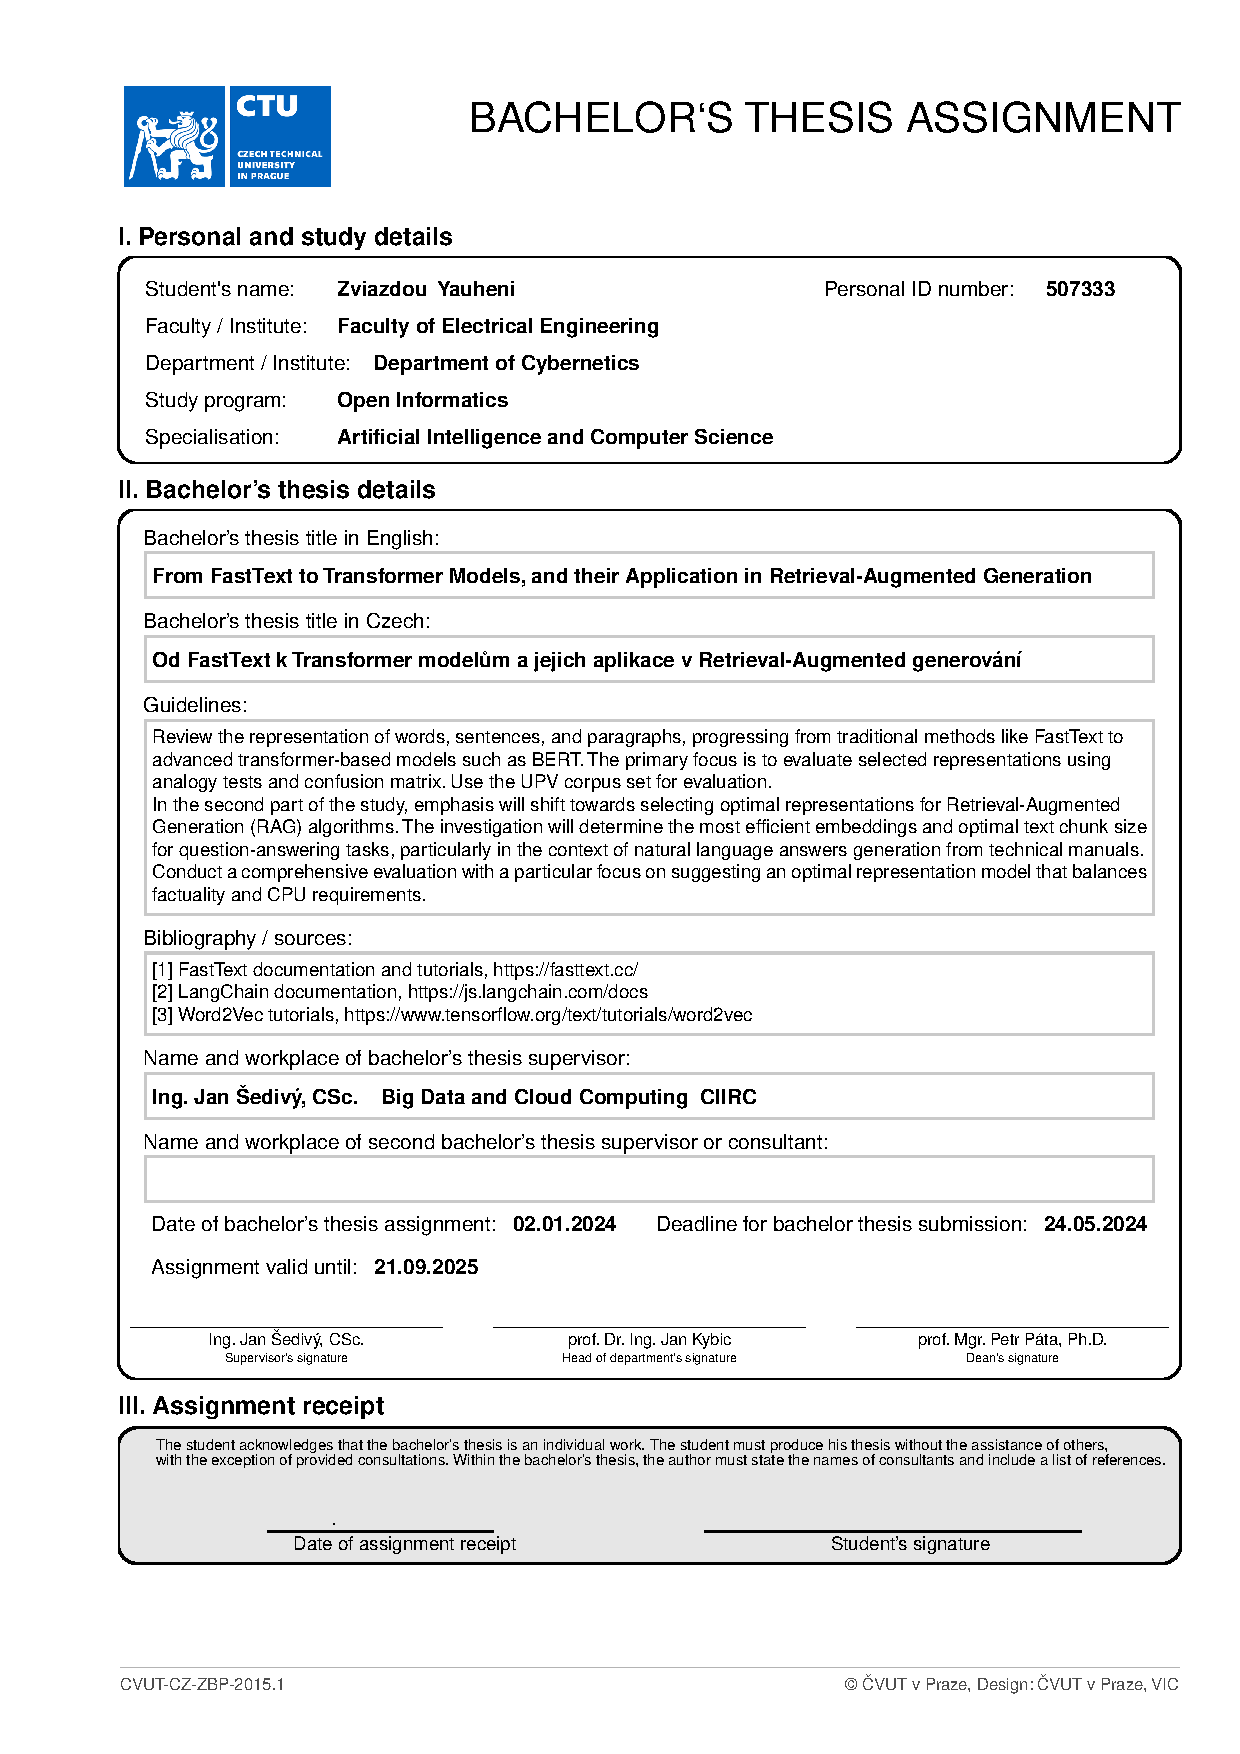
\includepdf{src/assignment.pdf}

%% --------------------------------------------------------------
%% |                         Declaration                        |
%% --------------------------------------------------------------

\conditionalClearPage

~\vfill{}

\section*{Declaration}

I declare that presented work was developed independently, and that I have listed all sources of information used within, in accordance with the Methodical instructions for ob-serving ethical principles in preparation of university theses.
I acknowledge the use of AI tools for rephrasing and grammatical correction.


\vspace{1.5cm}
~\\

In Prague 24.05.2024              \hfill{}                               Yauheni Zviazdou

\hfill{}~~~~~~~~~~~~~~~

\newpage{}


%% --------------------------------------------------------------
%% |                          Abstracts                         |
%% --------------------------------------------------------------

\conditionalClearPage

%!TEX root = ../main.tex

\begin{changemargin}{0.8cm}{0.8cm}

~\vfill{}

\section*{Abstract}
\vskip 0.5em

%The study of autonomous \acp{UAV} has become a prominent sub-field of mobile robotics.
This is en abstract.


\vskip 1em

{\bf Keywords} \Keywords

\vskip 2.5cm

\end{changemargin}

\acresetall

\conditionalClearPage

%!TEX root = ../main.tex

\begin{changemargin}{0.8cm}{0.8cm}

~\vfill{}

\section*{Abstrakt}
\vskip 0.5em

\sloppy
Výzkum na poli autonomních bezpilotních prostředků (UAV) se stal významným oborem mobilní robotiky.

\vskip 1em

{\bf Klíčová slova} \KlicovaSlova

\vskip 2.5cm

\end{changemargin}

\acresetall 

%% --------------------------------------------------------------
%% |                        Abbreviations                       |
%% --------------------------------------------------------------

\conditionalClearPage

\begin{changemargin}{0.8cm}{0.8cm}

~\vfill{}

\section*{Abbreviations}

% this will print only the used abbreviations
%!TEX root = ../main.tex

\begin{acronym}
  \acro{CTU}[CTU]{Czech Technical University}
  \acro{API}[API]{Application Programming Interface}
  \acro{RAG}[RAG]{Retrieval-Augmented Generation}
  \acro{NLP}[NLP]{Natural Language Procession}
  \acro{STS}[STS]{Semantic Textual Similarity}
  \acro{QA}[QA]{Question Answering}
  \acro{BERT}[BERT]{Bidirectional Encoder Representations from Transformers}
  \acro{CBOW}[CBOW]{Continuous Bag-of-Words}
  \acro{GloVe}[GloVe]{Global vectors}
  \acro{ML}[ML]{Machine Learning}
  \acro{NN}[NN]{Neural Network}
  \acro{BoW}[BoW]{Bag-of-Words}
  \acro{TF-IDF}[TF-IDF]{Term Frequency-Inverse Document Frequency}
  \acro{OOV}[OOV]{Out of vocabulary}
\end{acronym}


\vskip 2.5cm

\end{changemargin}

\conditionalClearPage

%% --------------------------------------------------------------
%% |                      Table of contents                     |
%% --------------------------------------------------------------

\tableofcontents

\conditionalClearPage

% set up the full page style with normal page numbering
\pagestyle{full}
\pagenumbering{arabic}

%% --------------------------------------------------------------
%% |                        Introduction                        |
%% --------------------------------------------------------------

%!TEX root = ../main.tex

\chapter{Introduction\label{chap:introduction}}

\section{Text representation}
The human language, with its nuances and complexities, presents a significant challenge for machines to understand.
\ac{NLP} bridges this gap, and at its core lies the critical concept of text representation.
This process acts as a translator, bridging the gap between the richness of text and the numerical language that machines understand.
By effectively capturing the meaning within words and their relationships, text representation empowers \ac{NLP} models to leverage machine learning's capabilities.
From sentiment analysis to machine translation, this ability to represent meaning fuels the advancements in \ac{NLP}, enabling machines to interact with and decipher human language with ever-increasing accuracy.

\section{Evolution of text representation methods}

\ac{NLP} has undergone a significant transformation in its approach to text representation.
Early methods, such as one-hot encoding, while simple to implement, suffered from limitations in efficiency due to dimensionality and sparsity issues.

Word embedding techniques (e.g., Word2Vec, \ac{GloVe}, FastText) offered a significant improvement by capturing semantic relationships between words through high-dimensional word vectors.
However, these techniques primarily focused on local context within a limited window, hindering their ability to capture complex relationships within sentences or documents.

The emergence of deep learning architectures, particularly transformer-based models like \ac{BERT}, revolutionized the field of text representation.
These models allows to not only understand the meaning of individual words but also consider their interaction and context within a sentence or document.

\begin{figure}
  \centering
  \begin{tikzpicture}
    %Nodes
    \begin{scope}[every node/.style={rectangle, draw=black, thick, align=left, minimum width=10em}]
    \node (Word2Vec)     []                  {Word2Vec};
    \node (GloVe)        [below=of Word2Vec] {\ac{GloVe}};
    \node (FastText)     [below=of GloVe]    {FastText};
    \node (Transformers) [below=of FastText] {Transformers};
    \end{scope}

    % Text labels (outside nodes)
    \node[right=of Word2Vec.east]     {2013};
    \node[right=of GloVe.east]        {2014};
    \node[right=of FastText.east]     {2016};
    \node[right=of Transformers.east] {2017};

    %Lines
    \draw[->] (Word2Vec.south) -- (GloVe.north);
    \draw[->] (GloVe.south)    -- (FastText.north);
    \draw[->] (FastText.south) -- (Transformers.north);
\end{tikzpicture}  
  \caption{Evolution of the text representation methods.}
  \label{fig:ecolution_text_representation}
\end{figure}

\section{Research objective}

This research aims to evaluate the effectiveness of various word, sentence, and paragraph representations for their subsequent application in \ac{RAG} algorithms, with a specific focus on the domain of technical \ac{QA}.

%% --------------------------------------------------------------
%% |                      Literature Review                     |
%% --------------------------------------------------------------

%!TEX root = ../main.tex

\chapter{Literature Review\label{chap:literature_review}}

\section{Traditional word embedding methods}

\subsection{Word2Vec}
Word2Vec \cite{mikolov2013efficient} is an algorithm that generates word embedding using information about the target word (context).
Word2Vec uses \ac{NN} and \ac{ML} techniques to generate word embedding for every word in vocabulary during training.
As \ac{NN} architecture is used \ac{CBOW} and Skip-gram, \reffig{fig:cbow_skipgram_scheme}.

\begin{figure}[h]
 \centering
    \begin{tikzpicture}[
    framed,
    squarednode/.style={rectangle, draw=black!60, very thick, minimum size=5mm},
    emptysquare/.style={squarednode, draw=none},
    largedrectangle/.style={squarednode, minimum width=10mm, minimum height=15mm},
    emptyrectangle/.style={squarednode, draw=none,minimum width=10mm},
    ]
    %Nodes
    \node[emptysquare]     (input3)  []                 {};
    \node[squarednode]     (input2)  [above=of input3]  {};
    \node[squarednode]     (input1)  [above=of input2]  {};
    \node[squarednode]     (input4)  [below=of input3]  {};
    \node[squarednode]     (input5)  [below=of input4]  {};
    \node[largedrectangle] (sum)     [right=of input3]  {SUM};
    \node[emptyrectangle]  (sum3)    [right=of input3]  {};
    \node[emptyrectangle]  (sum2)    [above=of sum3]    {};
    \node[emptyrectangle]  (sum1)    [above=of sum2]    {};
    \node[squarednode]     (output)  [right=of sum]     {};
    \node[emptysquare]     (output2) [above=of output]  {};
    \node[emptysquare]     (output1) [above=of output2] {};
    
    % Text labels (outside nodes)
    \node[left=of input1.east, xshift=3mm] {w(t-2)};
    \node[left=of input2.east, xshift=3mm] {w(t-1)};
    \node[left=of input4.east, xshift=3mm] {w(t+1)};
    \node[left=of input5.east, xshift=3mm] {w(t+2)};
    \node[below=of output.north]           {w(t)};
    \node[above=of input1.north]           {Input};
    \node[above=of sum1.north]             {Projection};
    \node[above=of output1.north]          {Output};

    %Lines
    \draw[->] (input1.east) -- (sum.west);
    \draw[->] (input2.east) -- (sum.west);
    \draw[->] (input4.east) -- (sum.west);
    \draw[->] (input5.east) -- (sum.west);
    \draw[->] (sum.east)    -- (output.west);
\end{tikzpicture}
    \begin{tikzpicture}[
    framed,
    squarednode/.style={rectangle, draw=black!60, very thick, minimum size=5mm},
    emptysquare/.style={squarednode, draw=none},
    largedrectangle/.style={squarednode, minimum width=10mm, minimum height=15mm},
    emptyrectangle/.style={squarednode, draw=none,minimum width=10mm},
    ]
    %Nodes
    \node[squarednode]     (input3)  []                 {};
    \node[emptysquare]     (input2)  [above=of input3]  {};
    \node[emptysquare]     (input1)  [above=of input2]  {};
    \node[emptysquare]     (input4)  [below=of input3]  {};
    \node[emptysquare]     (input5)  [below=of input4]  {};
    \node[largedrectangle] (sum)     [right=of input3]  {};
    \node[emptyrectangle]  (sum3)    [right=of input3]  {};
    \node[emptyrectangle]  (sum2)    [above=of sum3]    {};
    \node[emptyrectangle]  (sum1)    [above=of sum2]    {};
    \node[emptysquare]     (output3) [right=of sum]     {};
    \node[squarednode]     (output2) [above=of output3] {};
    \node[squarednode]     (output1) [above=of output2] {};
    \node[squarednode]     (output4) [below=of output3] {};
    \node[squarednode]     (output5) [below=of output4] {};
    \node[emptysquare]     (output1) [above=of output2] {};
    
    % Text labels (outside nodes)
    \node[below=of input3.north]  {w(t)};
    \node[right=of output1.west]  {w(t-2)};
    \node[right=of output2.west]  {w(t-1)};
    \node[right=of output4.west]  {w(t+1)};
    \node[right=of output5.west]  {w(t+2)};
    \node[above=of input1.north]  {Input};
    \node[above=of sum1.north]    {Projection};
    \node[above=of output1.north] {Output};

    %Lines
    \draw[->] (input3.east) -- (sum.west);
    \draw[->] (sum.east)    -- (output1.west);
    \draw[->] (sum.east)    -- (output2.west);
    \draw[->] (sum.east)    -- (output4.west);
    \draw[->] (sum.east)    -- (output5.west);
\end{tikzpicture}
 \caption{\ac{CBOW} and Skip-gram schemes respectively.}
    \label{fig:cbow_skipgram_scheme}
\end{figure} 

Due to its algorithmic simplicity and efficiency, Word2Vec has established itself as a strong baseline for numerous \ac{NLP} tasks.
Compared to more recent and complex models, Word2Vec requires minimal hyperparameter tuning, making it a relatively straightforward approach.

However, it is important to acknowledge that Word2Vec has limitations.
These include its inability to capture \textbf{global information} within a document, its challenges in effectively handling \textbf{morphologically rich languages} (languages with many word variations), and its lack of awareness of the \textbf{broader context} beyond a limited window of surrounding words.

\subsection{\acf{GloVe}}
\ac{GloVe} \cite{pennington2014glove} leverages the co-occurrence statistics of words within a corpus to learn vector representations.
This approach involves constructing a co-occurrence matrix, where each entry reflects the frequency of two words appearing together within a predefined window size.
This matrix essentially captures the relative importance of various word pairings.

A core principle of \ac{GloVe} lies in the notion that word vectors should effectively encode the ratios between co-occurrence probabilities of words.
By analyzing these ratios, \ac{GloVe} can identify semantic relationships between words.
This is achieved by factorizing the co-occurrence matrix into a lower-dimensional space, allowing for efficient representation and manipulation of word meanings.

To optimize the learned word embeddings, \ac{GloVe} employs a weighted least squares objective function.
This function aims to minimize the discrepancy between the dot product of two word vectors and the logarithm of their co-occurrence probability.
Through iterative adjustments of the word vectors, \ac{GloVe} converges on a solution that yields the desired word embeddings.

\subsection{FastText}
FastText \cite{bojanowski2017enriching} utilizes similar \ac{NN} architectures as Word2Vec, namely \ac{CBOW} and Skip-gram, but applies them to character n-grams (subwords) instead of entire words.
This decomposition allows FastText to represent a word's meaning by considering its constituent subword components.
Consequently, FastText offers advantages in two key areas:

\begin{itemize}
  \item \textbf{Rare Word Embeddings}:
    Unlike Word2Vec, which struggles with words appearing infrequently in the training data, FastText can construct meaningful representations for rare words.
    By leveraging known subwords, FastText can represent unseen words, making it particularly valuable for working with large and diverse datasets.    
  \item \textbf{Handling Morphologically Rich Languages}:
    Languages with complex morphology, where words are formed through prefixes and suffixes, often pose challenges for Word2Vec.
    FastText overcomes this limitation by capturing the shared subwords between derived words and their root forms.
    This allows FastText to represent the inherent relationships between words in these languages, leading to more accurate \ac{NLP} tasks.
\end{itemize}
However, it's important to acknowledge that FastText also has limitations:
\begin{itemize}
  \item \textbf{Context Insensitivity}:
    Similar to Word2Vec, FastText embeddings do not inherently capture the order or context in which words appear within a sentence.
    This can be a drawback for tasks like sentiment analysis or machine translation, where word order and context are crucial for accurate interpretation.
  \item \textbf{Limited Long-Range Dependency Capture}:
    While subwords allow FastText to capture local context, they might not effectively capture long-range dependencies within sentences.
    This can be a disadvantage for tasks requiring analysis of complex sentence structures, where understanding the relationships between words across larger distances is important.    
\end{itemize}

\section{Transformer-based models}
Transformer models \cite{vaswani2023attention} \nocite{umarjamilai} underpin powerful \ac{NLP} models like \ac{BERT}.
A key advantage is their self-attention mechanism, which assigns importance to words based on context, not just position.
This enables efficient parallel processing of entire sentences.
Architecture of transformers visualized in \reffig{fig:model-arch}.

\begin{figure}[h]
 \centering
 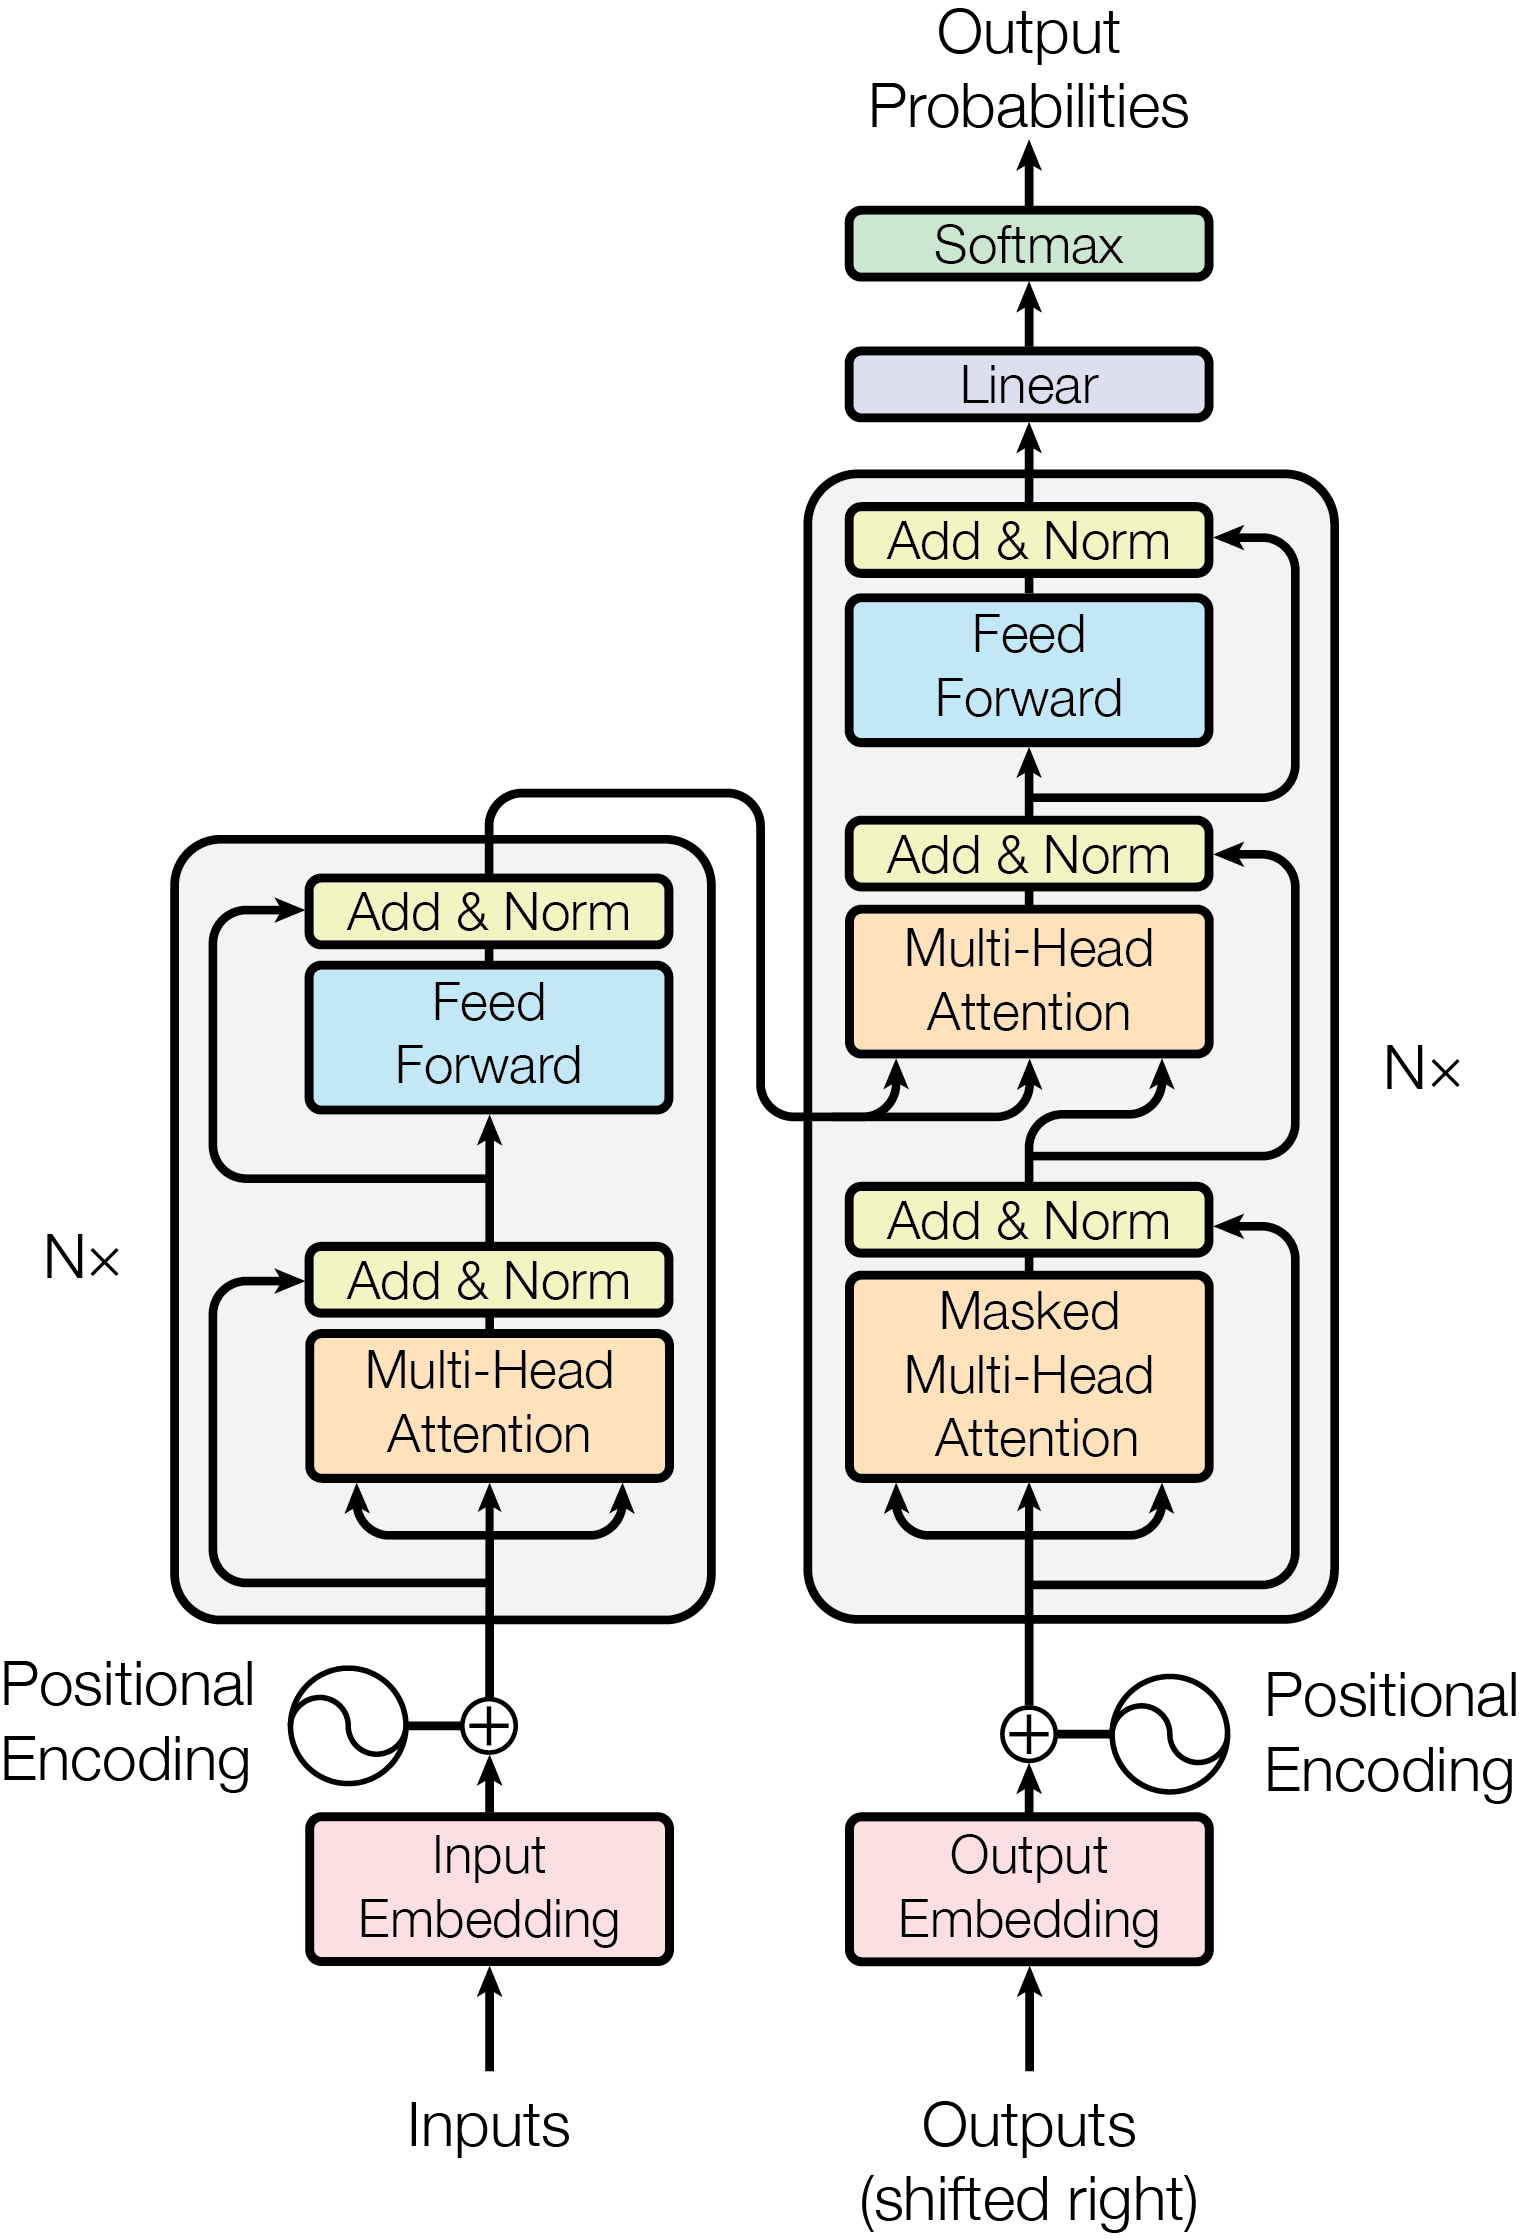
\includegraphics[scale=0.6]{src/fig/imgs/transformer_arch.png}
 \caption{The Transformer - model architecture.}
    \label{fig:model-arch}
\end{figure}

\ac{BERT} \cite{devlin2019bert} builds on transformers with pre-training on a massive text corpus.
\ac{MLM} and \ac{NSP} further enhance \ac{BERT}'s capabilities, fostering deep contextual understanding and grasp of sentence relationships.
\ac{MLM} injects a deeper understanding of context into \ac{BERT} by requiring it to predict masked words within a sentence.
Through this process, \ac{BERT} learns the relationships between words and their meaning based on the surrounding context.
This goes beyond simple memorization - it allows \ac{BERT} to grasp the nuances of language and handle even unseen words.
\ac{NSP}, on the other hand, strengthens \ac{BERT}'s ability to understand the flow and connection between sentences.
During training, \ac{BERT} is presented with sentence pairs and tasked with determining if the second sentence logically follows the first. 
By tackling this objective, \ac{BERT} develops a grasp of sentence relationships, enabling it to analyze and process text that unfolds across multiple sentences, like news articles or conversations.

These strengths make transformers, particularly \ac{BERT}, well-suited for \ac{NLP} tasks.
Their advantage lies in capturing contextual understanding, leading to richer text representations and superior comprehension of semantic relationships.

Furthermore, \ac{BERT} excels in transfer learning, readily adapting to various tasks (sentiment analysis, \ac{QA}) with minimal modifications.
Additionally, efficiency and speed are benefits due to parallel processing and pre-training.

The transformer model's effectiveness is validated by state-of-the-art performance across \ac{NLP} benchmarks.
Finally, \ac{BERT}'s robustness allows it to handle nuances in text without significant performance degradation.

\section{Methods of text representations evaluation}

\subsection{Analogy tests}

Analogy tests, as demonstrated in the seminal Word2Vec paper \cite{mikolov2013efficient}, is a widely used method for assessing the quality of text representations, particularly word embeddings.
These tests evaluate whether the semantic relationships between words are effectively captured and preserved within the vector space employed by the model.

A typical analogy test question follows the format "A is to B as C is to D," where A, B, C, and D represent words.
For instance, the question "man is to king as woman is to queen" probes the model's understanding of gender relations.
If the word embeddings are of high quality, performing the vector operation vector(king) - vector(man) + vector(woman) should result in a vector that closely resembles vector(queen).
This outcome indicates that the model has successfully learned the analogous relationship between "man" and "king" and "woman" and "queen".

\subsection{Confusion matrix}

Confusion matrices are a widely used tool for evaluating classification algorithms, and they can be adapted to assess text representations in tasks such as word sense disambiguation, part-of-speech tagging, or sentiment analysis.
A confusion matrix is a table that describes the performance of a classification model by comparing predicted and actual labels.

\section{\acf{RAG}}
\ac{RAG} \cite{lewis2021retrievalaugmented} \nocite{umarjamilai} is an advanced \ac{NLP} framework that combines the strengths of retrieval-based and generation-based models to produce high-quality, contextually relevant text based on the provided document (web-page, etc.), instruction and query (question). 

\subsection{Architecture of \ac{RAG}}
The \ac{RAG} algorithm leverages a two-stage approach for answer generation: retrieval and generation.
Both stages rely heavily on the chosen text representation technique.

\begin{itemize}
  \item \textbf{Retrieval}:
    In the initial phase, the algorithm extracts relevant information from the document and splits it into manageable chunks.
    These chunks are then fed into text representation models, which convert them into a format suitable for efficient retrieval.
    This process results in encoded representations of the information, which are then stored within a vector database.
    During the retrieval phase, \ac{RAG} utilizes the same text representation model to encode the user's query (question).
    Subsequently, it searches the vector database and identifies the top-$K$ most relevant passages based on their encoded representations.
  \item \textbf{Generation}:
    The $K$ retrieved passages identified in the information retrieval phase serve as crucial contextual information for the \ac{LLM} within the \ac{RAG} system.
    By providing this context alongside the user's question and any additional instructions, the \ac{LLM} is empowered to generate a comprehensive and informative answer.
\end{itemize}

The architecture of the \ac{RAG} algorithm is shown on the \reffig{fig:RAG_scheme}.

\begin{figure}[h]
 \centering
  % Inspired by:
% https://en.m.wikipedia.org/wiki/File:RAG_schema.svg
% https://github.com/hkproj/retrieval-augmented-generation-notes/blob/main/Slides.pdf

\begin{tikzpicture}[
    longnode/.style={rectangle, rounded corners=.5em, draw=black!60, very thick, align=left, minimum height=1.7em, minimum width=9em},
    emptylong/.style={longnode, draw=none},
    highnode/.style={longnode, minimum height=10.2em},
    line width=1pt, black
    ]
    
    %Nodes
    \node[longnode]  (question)    []                     {Question};
    \node[emptylong] (empty1)      [below=of question]    {};
    \node[longnode]  (embeddings1) [below=of empty1]      {Embeddings};
    \node[longnode]  (vector_db)   [right=of embeddings1] {Vector database};
    \node[longnode]  (embeddings2) [below=of vector_db]   {Embeddings};
    \node[longnode]  (chunks)      [below=of embeddings2] {Split into chunks};
    \node[longnode]  (documents)   [below=of chunks]      {Documents};
    \node[longnode]  (context)     [right=of vector_db]   {Context};
    \node[longnode]  (instruction) [above=of context]     {Instruction};
    \node[emptylong] (llm_empty3)  [right=of context]     {};
    \node[emptylong] (llm_empty2)  [above=of llm_empty3]  {};
    \node[emptylong] (llm_empty1)  [above=of llm_empty2]  {};
    \node[highnode]  (LLM)         [right=of instruction] {LLM};
    \node[longnode]  (answer)      [below=of llm_empty3]  {Answer};

    %Lines
    \draw[->] (question.south)    --                                                  (embeddings1.north);
    \draw[->] (embeddings1.east)  -- node[text width=3em,midway,above=0.7em] {Search} (vector_db.west);
    \draw[->] (embeddings2.north) -- node[text width=3em,midway,right=0.7em] {Store}  (vector_db.south);
    \draw[->] (chunks.north)      --                                                  (embeddings2.south);
    \draw[->] (documents.north)   --                                                  (chunks.south);
    \draw[->] (vector_db.east)    -- node[text width=3em,midway,above=0.7em] {Top-K}  (context.west);
    \draw[->] (context.east)      --                                                  (llm_empty3.west);
    \draw[->] (instruction.east)  --                                                  (llm_empty2.west);
    \draw[->] (question.east)     --                                                  (llm_empty1.west);
    \draw[->] (llm_empty3.south)  --                                                  (answer.north);
\end{tikzpicture}
 \caption{Retrieval-Augmented Generation architecture.}
  \label{fig:RAG_scheme}
\end{figure}

\subsection{Factors influencing \ac{RAG} performance}
The performance of \ac{RAG} systems can be influenced by several key factors.
Two important aspects are:

\begin{itemize}
  \item \textbf{Embedding Model Selection}:
    Previous work \cite{joshi2024RAGemb} suggests that the choice of the embedding model significantly impacts \ac{RAG} performance.
    Different embedding models offer varying strengths in capturing semantic relationships within text data.
    Selecting the most suitable model depends on the specific task and dataset.
  \item \textbf{Document Chunking Size}:
    Another factor influencing \ac{RAG} performance is the size of the document chunks used for retrieval \cite{theja2023RAGchunk}.
    Splitting documents into smaller chunks can potentially improve retrieval efficiency.
    However, excessively small chunks may lead to a loss of context and hinder the \ac{RAG} system's ability to generate coherent and relevant text.
    Finding the optimal chunking size requires careful consideration of the task and available computational resources.    
\end{itemize}




% Literature Review Structure
% \begin{itemize}
%     \item Discuss traditional word embedding methods like FastText and their limitations.
%     \item Explain the concept of transformer-based models like \ac{BERT} and their advantages for text representation.
%     \item Review related work on \ac{RAG} algorithms and their dependence on effective text representations. Discuss existing research on evaluating text representations using analogy tests and confusion matrices.
%     \item Briefly mention the UPV corpus set as the chosen evaluation benchmark.
% \end{itemize}

%% --------------------------------------------------------------
%% |                        Methodology                         |
%% --------------------------------------------------------------

%!TEX root = ../main.tex

\chapter{Methodology\label{chap:methodology}}

\section{Embedding methods evaluation process}

This work specifically targets the evaluation of word, sentence, and paragraph representation methods on datasets in the Czech language.
This focus on Czech allows for a deeper understanding of how these methods perform in a language with specific characteristics, such as a rich inflectional morphology and the presence of diacritics.

\subsection{Text Data Preparation}
In certain foreign languages, a common issue arises when individuals incorrectly write words by omitting diacritics or altering letters, \reffig{fig:diacritics_diacriticless}.
This problem is prevalent in social media, chatbots, and other informal written communications.
As a result, embedding models face challenges in comprehending text without diacritics (hereinafter diacriticless).
A potential solution involves adapting data representation to accommodate both formal and informal styles of writing.

\begin{figure}[h]
  \centering
  \begin{tikzpicture}
    %Nodes
    \begin{scope}[every node/.style={rectangle, draw=black!60, very thin, align=left, minimum width=12em, minimum height=1.7em}]
    \node (acute_diacritics)       []                             {á $\vert$ é $\vert$ í $\vert$ ó $\vert$ ú $\vert$ ý};
    \node (acute_diacriticless)    [right=of acute_diacritics]    {a $\vert$ e $\vert$ i $\vert$ o $\vert$ u $\vert$ y};
    \node (caron_diacritics)       [below=of acute_diacritics]    {č $\vert$ ď $\vert$ ě $\vert$ ň $\vert$ ř $\vert$ š $\vert$ ť $\vert$ ž};
    \node (caron_diacriticless)    [right=of caron_diacritics]    {c $\vert$ d $\vert$ e $\vert$ n $\vert$ r $\vert$ s $\vert$ t $\vert$ z};
    \node (overring_diacritics)    [below=of caron_diacritics]    {ů};
    \node (overring_diacriticless) [right=of overring_diacritics] {u};
    \end{scope}

    % Text labels (outside nodes)
    \node[left=of acute_diacritics.west]    {Acute:};
    \node[left=of caron_diacritics.west]    {Caron:};
    \node[left=of overring_diacritics.west] {Overring:};

    %Lines
    \draw[->] (acute_diacritics.east)    -- (acute_diacriticless.west);
    \draw[->] (caron_diacritics.east)    -- (caron_diacriticless.west);
    \draw[->] (overring_diacritics.east) -- (overring_diacriticless.west);
\end{tikzpicture}
  \caption{Usual changes in informal czech texts.}
  \label{fig:diacritics_diacriticless}
\end{figure} 

This study will employ two distinct text representations: text with diacritics and text without diacritics.
To ensure optimal evaluation, the diacritic text will be assessed using datasets that preserve these diacritics, while the diacriticless text will be evaluated using datasets that lack diacritics.

As detailed in \reflst{lst:diacriticless.sh}, this script is used for creating diacriticless versions of the datasets.

\begin{lstlisting}[language=bash,basicstyle=\small\ttfamily, frame=single, caption={Script for removing diacritics using Unix utilities}, captionpos=b, label={lst:diacriticless.sh},backgroundcolor=\color{light-gray}] 
  sed 's/.*/\L&/' "$1" | iconv -f utf-8 -t ascii//TRANSLIT > diacriticless/"$1"
\end{lstlisting}

\subsection{Evaluation  benchmark}

\subsubsection{UPV FAQ}

Dataset is comprised of frequently asked questions (FAQs) and their answers from the Industrial Property Office of the Czech Republic website \footnote{UPV website: \url{https://upv.gov.cz/}}, organized into four distinct groups, as detailed in \reftab{table:UPV_FAQ_info}.

This work will evaluate two key metrics using UPV FAQ dataset
\begin{itemize}
  \item \textbf{Question matching accuracy}:
    This metric involves calculating the cosine similarity between all possible question pairs within a dataset.
    A question is considered successfully matched if its second-highest cosine similarity score corresponds to another question belonging to the same class (i.e., the question with the highest similarity is likely the same question itself). 
    The overall question matching accuracy is then computed as the ratio of successfully matched questions to the total number of question pairs evaluated.  
  \item \textbf{Answer matching accuracy}:
    This metric assesses the system's ability to identify the correct answer for a given question.
    The system accomplishes this by directly comparing the question with pre-generated answer embeddings.
    By evaluating the similarity between the question and each answer embedding, the system classifies the question as corresponding to the answer with the highest similarity score.
    The overall answer matching accuracy is then calculated as the proportion of questions for which the system correctly identifies the corresponding answer.  
\end{itemize}

\begin{table}[!ht] 
    \centering   
    \begin{tabular}{ |p{2cm}||p{3cm}| }
        \hline
        Tests set & Number of tests \\
        \hline
        FAQv5     & 2054            \\
        FAQ50     & 561             \\
        FAQ76     & 2025            \\
        FAQ76v2   & 1965            \\
        \hline
        \hline
        All       & 6605            \\
        \hline
    \end{tabular}
    \caption{Information about UPV FAQ tests}
    \label{table:UPV_FAQ_info}
\end{table}

Traditional models will be assessed using jirkoada/upv\_faq \footnote{jirkoada/upv\_faq evaluator on github: \url{https://github.com/jirkoada/upv_faq}}, while transformer models will be evaluated using ezvezdov/upv\_faq\_transformers \footnote{ezvezdov/upv\_faq\_transformers evaluator on github: \url{https://github.com/ezvezdov/upv_faq_transformers}}.


\subsubsection{Analogies}

This study opted to exclude analogy-based evaluation methods for assessing the performance of transformer models.
This decision stems from the fundamental differences between traditional pre-trained models and transformer architectures in how they generate word embeddings.

Traditional models typically employ pre-training techniques that result in static word embeddings.
These embeddings capture comprehensive information about a word based on its occurrences throughout the training corpus.
This characteristic allows for the use of analogy tests where the model is presented with a triplet of words (e.g., "King" - "Man" + "Woman") and expected to predict the fourth word that completes the analogy ("Queen").

However, transformer models operate differently.
They generate word embeddings dynamically, considering the specific context in which a word appears within a sentence.
This context-dependent nature of transformer embeddings renders traditional analogy tests inapplicable.
Providing a single, isolated word to a transformer model would not be sufficient for it to generate a high-quality embedding that effectively captures all potential word contexts.

In light of these limitations, analogy-based evaluations are not well-suited for assessing the performance of transformer models.
Therefore, we opted to prioritize alternative evaluation methods that are more compatible with the context-aware embedding generation process employed by transformers.
These alternative methods, such as masked language modeling tasks, can provide a more accurate assessment of a transformer model's ability to capture semantic relationships within text.

\subsection{Baseline}
Due to the inherent morphological richness of the Czech language, this study adopts \textbf{FastText} as the baseline word embedding method.
This decision is motivated by FastText's ability to effectively capture morphological variations within words, a characteristic that has been shown to be advantageous for languages like Czech.
While other techniques like Word2Vec and \ac{GloVe} have been explored for word embedding generation, they have demonstrated lower performance in this context.
The FastText word embedding model will be trained using the fastText.cc library \footnote{fastText.cc library website: \url{https://fasttext.cc/}}

\subsubsection{Training parameters}
\begin{itemize}
  \item Architecture: \ac{CBOW} 
  \item Vector dimensionality: 300
  \item Loss function: Negative sampling loss
  \item Dictionary threshold (the frequency of the word to be included in the dictionary): 130
\end{itemize}

\subsubsection{Training data}

FastText model is trained on a segment of a preprocessed Common Crawl repository \cite{commoncrawl}, which encompasses raw data from web pages, as well as metadata and text extractions.
Given the nature of this dataset, it is expected to include misspellings and text lacking diacritics.

\begin{enumerate}
  \item Eliminating duplicate entries
  \item Filtering out lines containing fewer than 9 characters
  \item Excluding URLs
  \item Breaking lines into individual sentences
  \item Converting all text to lowercase
  \item Removing lines containing words exceeding 30 characters
  \item Excluding HTML tags with less than 100 characters
  \item Removing lines surpassing 500 characters
  \item Omitting words longer than 21 characters
\end{enumerate}

Processed corpus contains 3.87 billion words.

\subsubsection{Model summary}

The FastText models trained in this study exhibit differences in vocabulary size.
The diacritic model possesses a dictionary of approximately 800,000 words, while the diacriticless model contains roughly 762,000 words.
This discrepancy reflects the inherent reduction in word count due to the removal of diacritics in the diacriticless dataset.

These vocabulary sizes directly influence the number of trainable parameters within each model.
The number of parameters ($N$) can be calculated using the formula~\refeq{eq:cbow_parameters}.

\begin{align} \label{eq:cbow_parameters}
  & N = V_{\text{size}}d + d \\
  \text{where} \quad & V_{\text{size}} \text{ is model vocabulary size}  \notag \\
                      & d \quad \text{is chosen dimensionality of word embeddings} \notag
\end{align}
  
Applying this formula to the vocabulary sizes of our models:
\begin{itemize}
  \item The diacritics model possesses approximately 240 million parameters.
  \item The diacriticless model has approximately 229 million parameters.
\end{itemize}

\subsection{Chosen transformer models}
To ensure a comprehensive evaluation, a curated selection of embedding models will be utilized.
This selection encompasses three distinct categories:

\begin{enumerate}
  \item \textbf{Existing Czech Embedding Models}:
    This category incorporates established Czech embedding models developed within the Czech NLP community.
    Their inclusion allows for a focused analysis of how these models perform specifically for the Czech language.
  \item \textbf{Multilingual Models from the \ac{MTEB}}:
    The evaluation will leverage highly regarded multilingual models readily available through the \ac{MTEB}.
    This inclusion enables an assessment of how these models generalize to the Czech language, providing insights into their adaptability across languages.
  \item \textbf{Popular Monolingual Models from the \ac{MTEB} (rank is lower than 50)}:
    In addition to multilingual models, this selection will also include well-regarded monolingual models (models trained on a single language) from the \ac{MTEB}.
    This allows for a comparative analysis of how these models, potentially trained on English or other high-resource languages, perform on the Czech dataset.
\end{enumerate}

To ensure transparency, reproducibility, and foster community development, this study will exclusively evaluate open-source text embedding models.  Furthermore, to prioritize computational efficiency and applicability to our research setting, we will restrict our evaluation to models with a parameter size of less than 1 billion.
In cases where a model suite offers both monolingual and multilingual versions, we will prioritize the multilingual version for evaluation. This choice aligns with our focus on tasks that may involve processing text data in multiple languages, including Czech.

For a comprehensive overview of the chosen models' architectural details, please refer to Appendix~\ref{chap:appendix_A}.
This appendix provides a more in-depth examination of the specific configurations employed by each model.

% Czech models
%%%%%%%%%%%%%%%%%%%%%%%%%%%%%%%%%%%%
% Czert
\subsubsection{Czert-B} \label{modelczert-b}

The Czert model \cite{sido2021czert} is a set of Czech \ac{BERT}-like language representation models developed specifically to enhance performance in processing the Czech language.
These models leverage the \ac{BERT} and A Lite \ac{BERT} (ALBERT) \cite{lan2020albert} architectures and are designed to outperform multilingual models by training exclusively on Czech data.
The training set includes a comprehensive corpus of Czech texts, such as Wikipedia articles, news, and other texts, accumulating to around 36GB of data.

There are 2 variants of the Czert model, Czert-A and Czert-B. Unfortunately Czert-A model is not available, so we will test only Czert-B model.
Czert-B model is based on the traditional \ac{BERT} architecture (110M parameters).
Model are pre-trained from scratch using \ac{MLM} and \ac{NSP} tasks. However, a slight modification is made to the \ac{NSP} task to adapt it better to the Czech language corpus structure.

% Seznam
\subsubsection{Seznam's models} \label{model:seznam}
This study leverages a group of compact word embedding models specifically designed for the Czech language.
These models were developed by the Seznam research group with a focus on efficient word representation generation \cite{bednář2023like}.

\begin{itemize}
  \item \textbf{RetroMAE-Small}:
    This model leverages a \ac{BERT}-small architecture pre-trained with the \ac{RetroMAE} objective \cite{xiao2022retromae} on a custom Czech corpus.
    The \ac{RetroMAE} objective focuses on enhancing the model's ability to learn from \ac{MLM} tasks.
  \item \textbf{Dist-MPNet-ParaCrawl} \& \textbf{Dist-MPNet-CzEng}:
    These models are distilled versions of the \textit{sentence-transformers/all-mpnet-base-v2} \footnote{\label{hf_all-mpnet-base-v2} Model on the huggingface website: \url{https://huggingface.co/sentence-transformers/all-mpnet-base-v2}} using a knowledge distillation approach.
    Distillation involves training a smaller model (\ac{BERT}-small in this case) to mimic the performance of a larger, pre-trained model (\textit{sentence-transformers/all-mpnet-base-v2} \footref{hf_all-mpnet-base-v2}).
    The two distilled models differ in their training data: Dist-MPNet-ParaCrawl utilizes the parallel cs-en dataset from ParaCrawl \cite{espla2019paracrawl}, while Dist-MPNet-CzEng leverages the parallel cs-en dataset CzEng \cite{kocmi2020announcing}.
  \item \textbf{SimCSE-RetroMAE-Small} \& \textbf{SimCSE-Dist-MPNet-ParaCrawl} \& \textbf{SimCSE-Dist-MPNet-CzEng}:
    These models are based on the previously described RetroMAE-Small, Dist-MPNet-ParaCrawl, and Dist-MPNet-CzEng models respectively.
    Each is further fine-tuned with the \ac{SimCSE} objective \cite{gao2022simcse}.
    \ac{SimCSE} focuses on improving sentence embedding quality by encouraging models to generate similar representations for semantically equivalent sentences.
  \item \textbf{SimCSE-Small-E-Czech}:
    This model builds upon the Czech ELECTRA model \cite{kocián2021siamese}.
    It is fine-tuned with the \ac{SimCSE} \cite{gao2022simcse} objective to enhance the quality of its sentence embeddings.    
\end{itemize}

The developed models are about eight times smaller and five times faster than conventional base-sized models, making them suitable for real-time applications where computational efficiency is critical.
The models are trained using techniques like pre-training, knowledge distillation, and unsupervised contrastive fine-tuning to adapt to the limited availability of labeled Czech data.


% Multilingual models
%%%%%%%%%%%%%%%%%%%%%%%%%%%%%%%%%%%%
% mBERT
\subsubsection{mBERT} \label{model:mbert}
\ac{mBERT} \cite{devlin2019bert} leverages the same transformer-based architecture as the original \ac{BERT} model but boasts an increased number of parameters (178M) to enhance its capabilities.
A key distinction of \ac{mBERT} lies in its ability to understand and process text data across multiple languages.
To achieve this multilingual proficiency, \ac{mBERT} is trained on a massive dataset sourced from Wikipedia entries in 104 different languages.
This corpus is meticulously constructed to ensure balanced representation, meaning each language is included regardless of the size or depth of its corresponding Wikipedia.
This approach ensures that even languages with limited resources are adequately represented within the training data, fostering better performance for these languages.

% mE5
\subsubsection{\ac{mE5}} \label{model:me5}
\ac{mE5} models by Microsoft \cite{wang2024multilingual} are advanced text embedding models designed to operate across multiple languages based on English-only E5 models \cite{wang2024text}.
These models are available in three variants — small, base, and large — catering to different computational efficiency and performance needs.
The \ac{mE5} models are trained using a two-phase approach.
The first phase involves weakly-supervised contrastive pre-training on about 1 billion text pairs sourced from diverse multilingual corpora (Wikipedia, mC4, Multilingual CC News, Reddit, etc.).
The second phase is supervised fine-tuning on approximately 1.6 million data points from high-quality labeled datasets (MS MARCO \cite{bajaj2018ms}, Natural Questions (NQ) \cite{kwiatkowski2019natural}, TriviaQA \cite{joshi2017triviaqa}, SQuAD \cite{rajpurkar2016squad}, etc.).

% LaBSE
\subsubsection{LaBSE} \label{model:labse}
\ac{LaBSE} model \cite{feng2022languageagnostic}, developed by Google, is a state-of-the-art model for generating sentence embeddings that are effective across 109 languages.
It leverages the transformer architecture and is trained on both monolingual (from sources like CommonCrawl \cite{commoncrawl} and Wikipedia) and bilingual data (mined from web pages).
LaBSE utilizes a dual-encoder structure with \ac{BERT}-based encoding modules.
This setup enables the efficient processing of text pairs in multiple languages.

% XLM-R
\subsubsection{XLM-R} \label{model:xlm-roberta}
The \ac{XLM-R} model \cite{conneau2020unsupervised} is a significant advancement in unsupervised cross-lingual representation learning, introduced by Facebook AI.
It is specifically designed to improve performance across a wide range of cross-lingual tasks.
\ac{XLM-R} is pre-trained on a dataset dubbed 'CC-100', derived from Common Crawl \cite{commoncrawl}, covering about 2.5 terabytes of text across 100 languages.
This dataset is significantly larger than the ones used by its predecessors, offering a broader and more diverse linguistic foundation.

% SentenceTransformers
\subsubsection{SentenceTransformers models} \label{model:st-multilingual}

This work leverages SentenceTransformers \cite{reimers2019sentencebert}, a Python framework offering a comprehensive collection of pre-trained models designed for state-of-the-art sentence, text, and image embeddings.
These models are specifically tuned for various tasks, providing researchers with a powerful starting point for their investigations.

The following pre-trained models from SentenceTransformers will be evaluated in this study:
\begin{itemize}
  \item \textbf{Distiluse-Base-Multilingual-Cased-v2}:
    This model leverages knowledge distillation, a technique for creating a smaller and faster model by capturing the knowledge from a larger, pre-trained model.
    In this case, it is a distilled version of the multilingual Universal Sentence Encoder \cite{yang2019multilingual}.
    Notably, this version supports sentence encoding for over 50 languages, including Czech.
  \item \textbf{Paraphrase-Multilingual-MiniLM-L12-v2}: This pre-trained model focuses on paraphrase identification.
    It is a multilingual version of the \textit{sentence-transformers/paraphrase-MiniLM-L12-v2} \footnote{Model on the huggingface website: \url{https://huggingface.co/sentence-transformers/paraphrase-MiniLM-L12-v2}} model, trained on parallel datasets encompassing over 50 languages, including Czech.
    By learning paraphrase relationships, this model can potentially capture semantic similarities between sentences.
  \item \textbf{Paraphrase-Multilingual-MPNet-Base-v2}: Similar to the previous model, this is a multilingual version of the \textit{sentence-transformers/paraphrase-mpnet-base-v2} \footnote{ Model on the huggingface website: \url{https://huggingface.co/sentence-transformers/paraphrase-mpnet-base-v2}} model, trained on parallel data for over 50 languages, including Czech.
    This model is also designed for paraphrase identification, potentially aiding in tasks that require an understanding of semantic equivalence across sentences.
\end{itemize}


% Monolingual models
%%%%%%%%%%%%%%%%%%%%%%%%%%%%%%%%%%%%

% UAE-Large-V1
\subsubsection{UAE-Large-V1} \label{model-uae-large-v1}
The UAE-Large-V1 model \cite{li2024angleoptimized} focuses on enhancing short and long \ac{STS} tasks through a novel angle-optimized text embedding approach (AnglE) that works by dividing text embeddings into real and imaginary components in a complex space.
This model is designed to address the challenges posed by the saturation zones of the cosine function, which can impede learning by causing vanishing gradients.

The model is trained using a hybrid objective that combines cosine similarity, in-batch negatives, and angle differences in complex space.
This approach helps overcome the limitations of traditional cosine similarity measures by ensuring better gradient flow during training.
Training dataset includes around 21K samples and is specifically designed to evaluate \ac{STS} performance on long texts, which are common in real-world applications.

% Mxbai embed
\subsubsection{Mxbai embed}
This is study incorporates two models developed by MixedBread AI, mxbai-embed-large-v1 and mxbai-embed-2d-large-v1. 
\begin{itemize}
  \item \textbf{Mxbai-Embed-Large-v1} \cite{emb2024mxbai}:
    This model stands out as a high-performance English embedding model specifically designed for \ac{RAG} systems.
    As of March 2024, it holds the leading position among publicly available models of its class within the \ac{MTEB}.
    Notably, Mxbai-Embed-Large-v1 surpasses other models in tasks such as classification, clustering, and retrieval.
    The success of this model can be attributed to its robust training methodology.
    Mxbai-Embed-Large-v1 is trained on a massive dataset exceeding 700 million text pairs using a contrastive learning approach.
    This approach focuses on maximizing the similarity between semantically similar texts while contrasting dissimilar ones.
    Furthermore, the model undergoes fine-tuning with 30 million high-quality triplets leveraging the AnglE loss function.
    This fine-tuning step further refines the model's ability to distinguish semantic relationships within text data
  \item \textbf{Mxbai-Embed-2D-Large-v1} \cite{emb2024mxbai2d}:
    This model introduces a novel 2D-Matryoshka architecture \cite{li20242d}, marking a significant advancement in the field of text embedding.
    The 2D-Matryoshka architecture offers a key advantage over traditional approaches: it allows for both dimensionality reduction of embeddings and chunking of model layers.
    This  flexibility enables users to tailor the model size and complexity based on their specific computational needs.
    This allows for a crucial trade-off between computational efficiency and accuracy in resource-constrained environments.
    The model was designed to address the limitations of traditional dense embedding models, which produce fixed-size embeddings.
    These fixed-size embeddings can be inefficient for tasks requiring rapid processing or limited memory footprints.
    Mxbai-Embed-2D-Large-v1 tackles this challenge by employing a novel training strategy.
    This strategy incorporates contrastive training on a diverse dataset and fine-tuning on high-quality triplets.
    This approach allows the model to achieve competitive performance while offering significant reductions in resource consumption compared to traditional dense models.
\end{itemize}

% Nomic Embed
\subsubsection{Nomic-Embed-v1 and Nomic-Embed-v1.5} \label{model:nomic-embed}
The Nomic model \cite{nussbaum2024nomic}, designed for reproducible long-context text embedding, employs a modified BERT architecture optimized for 8192 token sequences.
It includes innovations such as rotary positional embeddings and SwiGLU activations, enhancing its ability to process longer texts.
The model undergoes a comprehensive training regime starting with unsupervised contrastive pretraining on large-scale datasets, followed by supervised fine-tuning using human-annotated data.
This process leverages contrastive learning to improve text embedding capabilities, significantly enhancing performance on both short and long-context tasks.

Nomic Embed v1.5 is an improvement upon Nomic Embed v1 that utilizes Matryoshka Representation Learning \cite{kusupati2024matryoshka} which gives developers the flexibility to trade off the embedding size for a negligible reduction in performance.

% GTE
\subsubsection{GTE and GTE-v1.5} \label{model:gte}
The \ac{GTE} model is a pivotal development in \ac{NLP}, utilizing a deep Transformer encoder based on a \ac{BERT}-like architecture for generating dense text embeddings.
Initially, the \ac{GTE} model is unsupervisedly pre-trained on approximately 800 million text pairs from diverse web sources, enabling broad semantic coverage.
It then undergoes supervised fine-tuning with 3 million annotated text triples from varied datasets, including MS MARCO and Natural Questions, applying contrastive learning to enhance text relevance detection and similarity assessments.
This dual-stage training strategy equips the \ac{GTE} model to excel in complex \ac{NLP} tasks, demonstrating significant versatility and robust performance across multiple applications.

There is also updated version \ac{GTE}-v1.5.

% BGE
\subsubsection{BGE-v1.5} \label{model:bge}
\ac{BGE} Models \cite{xiao2024cpack} are built on a BERT-like architecture, available in three sizes: small, base, and large.
They are trained using a sophisticated multi-stage process involving pre-training on large unlabeled data, contrastive learning for fine-tuning on text pairs, and multi-task learning with high-quality labeled datasets.
This training regimen equips BGE models to handle a wide range of text embedding tasks with high efficiency and accuracy.

% GIST-Embedding-v0
\subsubsection{GIST-Embedding-v0}
This study incorporates the GIST-Embedding-v0 suite of models, developed using the "Guided In-sample Selection of Training Negatives for Text Embedding Fine-tuning" (GIST) technique \cite{solatorio2024gistembed}.
These models leverage pre-trained models as a foundation and are then fine-tuned on specific datasets.

The fine-tuning process for GIST-Embedding-v0 utilizes the MEDI datasets \cite{su2023embedder}, which are further enhanced by the inclusion of mined triplets derived from the \ac{MTEB} Classification training dataset.
This targeted augmentation strategy aims to improve the model's performance on specific tasks.

Based on their performance in the \ac{MTEB}, our evaluation will focus solely on the GIST-Embedding-v0 models built upon the \ac{BGE}-v1.5 architecture (small, base, and large sizes).
This selection ensures we investigate the most promising fine-tuning approaches within the GIST-Embedding suite.

% TaylorAI
\subsubsection{TaylorAI tiny models} \label{model:taylorai}
This study incorporates two distilled transformer models from TaylorAI for evaluation:

\begin{itemize}
  \item \textbf{TaylorAI/BGE-micro-v2} \footnote{TaylorAI/bge-micro-v2 model on the huggingface website: \url{https://huggingface.co/TaylorAI/bge-micro-v2}}:
    This model is a 2-step distilled version of the small \ac{BGE}-v1.5 model
  \item \textbf{TaylorAI/GTE-tiny} \footnote{TaylorAI/gte-tiny model on the huggingface website: \url{https://huggingface.co/TaylorAI/gte-tiny}}:
    This model is a distilled version of the small version of \ac{GTE} model
\end{itemize}

% ember-v1
\subsubsection{Ember-v1}
This study leverages the Ember-v1 model, developed by LLMRails.
Ember-v1 is a text embedding model trained on a comprehensive dataset of text pairs encompassing a wide range of domains such as finance, science, medicine, law, and beyond.
Notably, the training process incorporates techniques inspired by both RetroMAE \cite{xiao2022retromae} and SetFit \cite{tunstall2022efficient}. 


% Snowflake-Arctic-Embed
% \subsubsection{Snowflake-Arctic-Embed} \label{model:snowflake-embed}
% This study investigates the use of Snowflake-Arctic-Embed, a suite of text embedding models optimized for retrieval tasks.
% The suite offers multiple model sizes (xs, s, m, m-long, l) for flexibility.

% Snowflake-arctic-embed leverages a two-stage training pipeline
% \begin{enumerate}
%   \item Pretraining on large batches of query-document pairs with dynamically generated negative examplesusing dataset with 400M samples combining public data and proprietary web search data.
%   \item Fine-tuning the model on a smaller dataset (1M samples) consisting of query-positive document-negative document triplets to improve retrieval accuracy.
% \end{enumerate}





% TODO:
% \subsubsection{jina-embeddings}
%Only jina-embeddings-v2, because it's better in \ac{MTEB}

\section{Optimizing Text Representations for \ac{RAG} in Technical \ac{QA}}

\subsection{Key factors}
To identify the most suitable text representation model for \ac{RAG} in technical \ac{QA}, we propose a comprehensive evaluation approach that considers the following key factors:

\begin{itemize}
  \item \textbf{Embedding Efficiency}:
    Computational efficiency is crucial for real-world applications.
    We will evaluate the processing time required for different representation models, considering factors like embedding dimensionality and model complexity.
    This ensures the chosen model can handle real-time \ac{QA} tasks within reasonable processing time constraints.
  \item \textbf{Text Chunk Size}:
    The size of text chunks used by the \ac{RAG} algorithm (e.g., words, sentences, or paragraphs) can impact performance.
    We will investigate the optimal chunk size for technical \ac{QA} tasks.
    Here, we will balance the granularity of information retrieved by the model with computational efficiency.
    Smaller chunks (words) might capture finer details but require more processing, while larger chunks (paragraphs) might be faster to process but might miss relevant details.  
  \item \textbf{Factuality of Generated Answers}:
    The primary objective is to generate answers that are factually accurate and consistent with the technical document.
    We will evaluate the models based on metrics that assess the factual correctness and coherence of the generated answers in response to technical questions.
    This ensures the generated answers are reliable and trustworthy for the user.
\end{itemize}

\subsection{Chunk Size and K Parameter Selection}
This section explores the selection of chunk sizes and the corresponding K parameter for evaluation using the \ac{RAG} model.
The chunk size refers to the length of text passages (number of characters) that will be processed by the \ac{RAG} model during evaluation.
The K parameter, on the other hand, determines the number of retrieved passages that the \ac{RAG} model will consider when generating a response.
Chosen parameters are shown at \reftab{table:RAG_settings}

\begin{table}[!ht] 
    \centering   
    \begin{tabular}{|l|c|c|}
        \hline
        Chunk size & $K$ \\
        \hline
        256        & 12  \\
        512        & 6   \\
        1024       & 3   \\
        2048       & 2   \\
        4096       & 1   \\
        \hline
    \end{tabular}
    \caption{Chunk sizes and corresponding $K$ parameter.}
    \label{table:RAG_settings}
\end{table}

\subsection{RAG pipeline}

This section describes the evaluation methodology employed for the \ac{RAG} model using an English language test set.
Due to limitations in the availability of Czech language testing data, we opted to utilize a private technical English data corpus for this evaluation.

The test set comprises two components: a technical manual and a set of 200 questions designed to assess document information retrieval capabilities.

For the embedding generation stage within \ac{RAG}, we will leverage the GTE\textsubscript{Small} model as popular small model with good \ac{MTEB} rating.

For the \ac{LLM} component of \ac{RAG}, we will utilize GPT-3.5-turbo \cite{brown2020language}.

The evaluation will be conducted using the jirkoada\/qa\_evaluator \footnote {jirkoada/qa\_evaluator on github: \url{https://github.com/jirkoada/qa_evaluator}} tool.


\subsection{Experiment hardware}
The computational workload was handled by an Intel Core i7-8550U CPU.
This is a 14nm mobile processor featuring 4 cores and 8 threads with a base clock of 1.8 GHz and a turbo boost frequency of 4.0 GHz.



% \section{Methodology structure}
% \begin{itemize}
%     \item Describe the evaluation process for different text representations.
%       \begin{itemize}
%         \item{Specify the chosen word, sentence, and paragraph representation models (e.g., FastText, BERT variants).}
%         \item{Explain the usage of analogy tests and confusion matrices for evaluation.}
%         \item{Detail the selection process for the UPV corpus set and its suitability for technical \ac{QA} tasks.}
%       \end{itemize}
%     \item Outline the second part of the study focusing on \ac{RAG} for technical QA.
%       \begin{itemize}
%         \item{Explain the \ac{RAG} algorithm and its reliance on text representations.}
%         \item{Describe the evaluation approach for selecting optimal representations for RAG.}
%         \item{Mention the factors considered during evaluation, such as embedding efficiency, text chunk size, and factuality of generated answers.}
%       \end{itemize}
% \end{itemize}

%% --------------------------------------------------------------
%% |                  Experiments and Results                   |
%% --------------------------------------------------------------

%!TEX root = ../main.tex

\chapter{Experiments and Results DRAFT\label{chap:experiments_and_results}}

\section{Text representation models}
Table \ref{tab:evaluatinon} presents the evaluation results for the chosen text embedding models.

\subsection{Analysis of results}
\subsubsection{Czech models}
Among the evaluated Czech models, SimCSE-RetroMAE-Small demonstrated the most promising performance.
This model effectively handled both text with diacritics and diacriticless variants, outperforming other models within this category.
Notably, the remaining Czech models achieved performance below the established baseline.

The performance of Czert-B can potentially be attributed to the fact that it was not specifically fine-tuned for the task of generating text embeddings.
This highlights the importance of fine-tuning models for the specific task at hand to optimize their performance.

Regarding the Seznam models, the observed differences in results likely stem from variations in their training processes.
The SimCSE-RetroMAE-Small model emerged as the clear leader within this group, suggesting that the fine-tuning strategy employed with \ac{SimCSE} and \ac{RetroMAE} may be particularly effective for these models.

\subsubsection{Multilingual models}
Among the evaluated multilingual models, all versions of mE5 and LaBSE demonstrated particularly promising performance.
Notably, mE5 achieved the highest overall results within the tested models.
Confusion matrices of evaluation are shown at \reffig{fig:Confusion_matrices}.
This suggests that the training objectives and architectures employed for these models might be well-suited for capturing semantic similarity across languages, including Czech.

Paraphrase-Multilingual-MiniLM-L12-v2 and Paraphrase-Multilingual-MPNet-Base-v2 exhibited strong performance when applied to text containing diacritics.
However, their performance appeared less effective when handling diacriticless text.
This observation suggests that these models might benefit from further training or adaptation specifically tailored for handling variations in Czech text with and without diacritics.

While mBERT and XLM-R did not achieve the same level of success as other models, it's important to acknowledge that the unsupervised training methods they employ (e.g. \ac{MLM} and \ac{NSP}) might not be specifically optimized for the task of assessing semantic similarity.
Alternative training objectives or supervised learning approaches tailored for this task might lead to improved performance from these models in the context of Czech text analysis.

\subsubsection{Monolingual models}

While all monolingual models achieved performance near the established baseline, this is a noteworthy finding considering they were not specifically trained on the Czech language.
This suggests that some level of semantic similarity can be captured between languages with inherent structural similarities, even without targeted training on the target language.
However, it is important to acknowledge that languages possess distinct vocabularies, grammatical structures, and cultural nuances.
Models trained solely on a language like English may struggle to fully grasp the intricacies of Czech text, potentially hindering their ability to achieve optimal performance in tasks involving semantic similarity assessment.

In contrast, several monolingual models, particularly the Nomic Embed models, the small version of GTE, and the large version of GTE-v1.5, exhibited performance exceeding the baseline.
This highlights the potential effectiveness of certain model architectures, even when not specifically trained on the target language.
Further investigation into the specific characteristics of these models that contribute to their success in this context might provide valuable insights for future research.

\begin{figure}[htbp]
    \centering

    \subfloat[Evaluatinon using diacritics tests.]{%
        \centering
        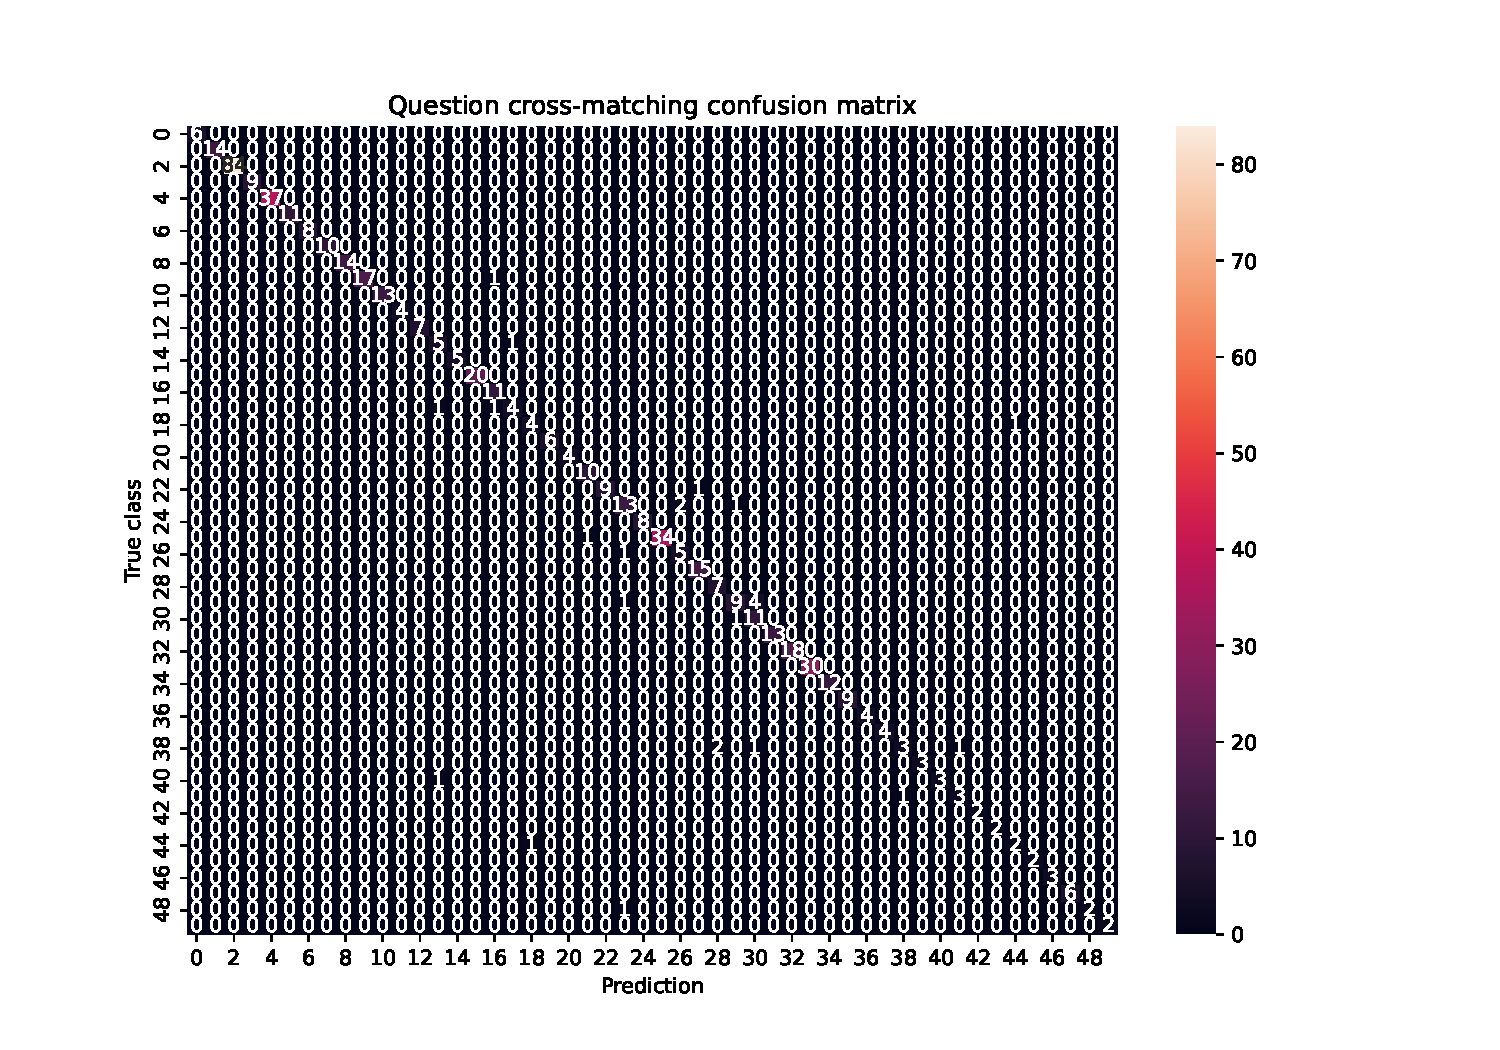
\includegraphics[width=0.54\textwidth,valign=t]{src/fig/pdfs/CM_QMA_FAQ50_diacritics.pdf}
        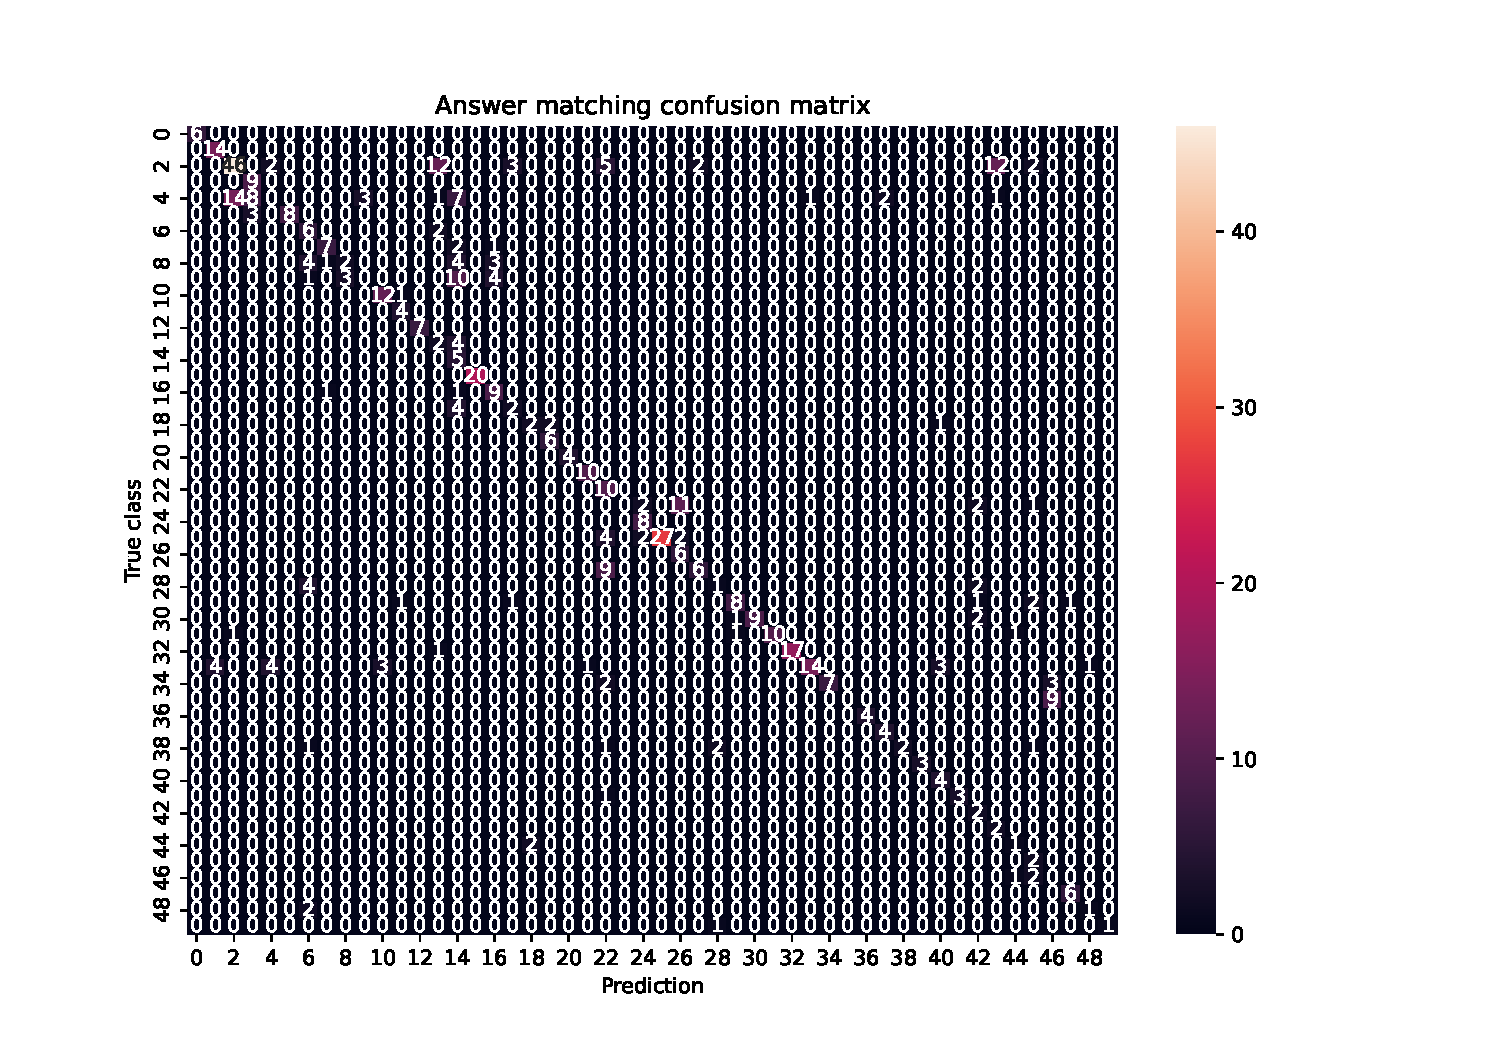
\includegraphics[width=0.54\textwidth,valign=t]{src/fig/pdfs/CM_AMA_FAQ50_diacritics.pdf}
        \label{fig:CM_diacritics}
    }

    \subfloat[Evaluatinon using diacriticless tests.]{%
        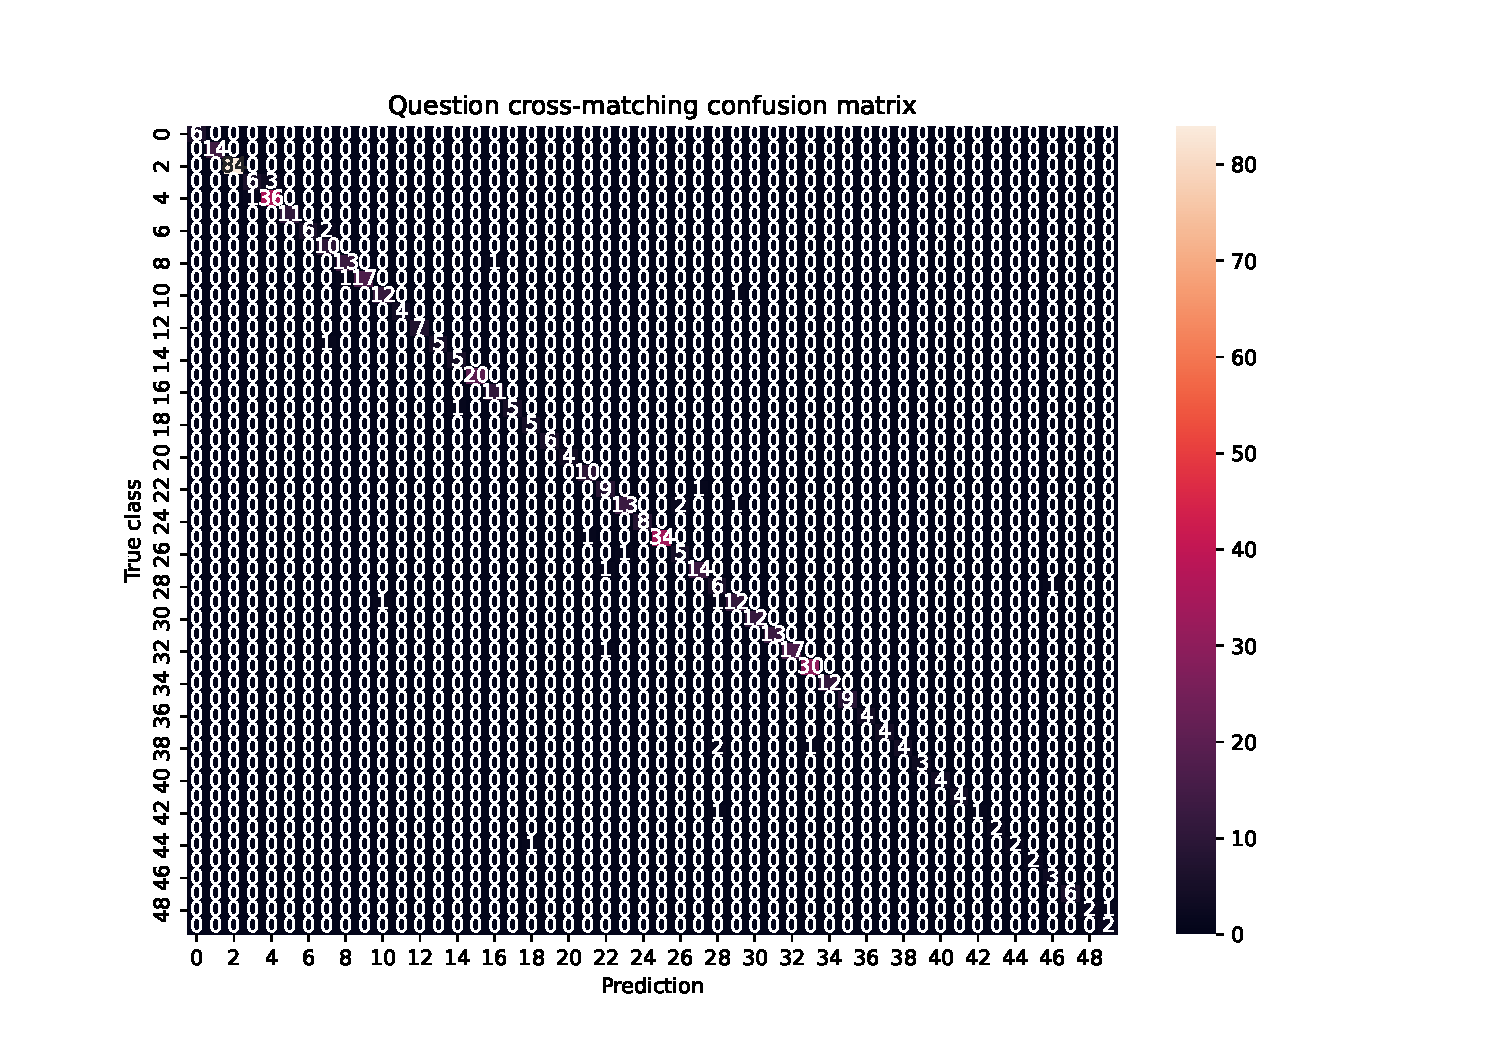
\includegraphics[width=0.54\textwidth,valign=t]{src/fig/pdfs/CM_QMA_FAQ50_diacriticless.pdf}
        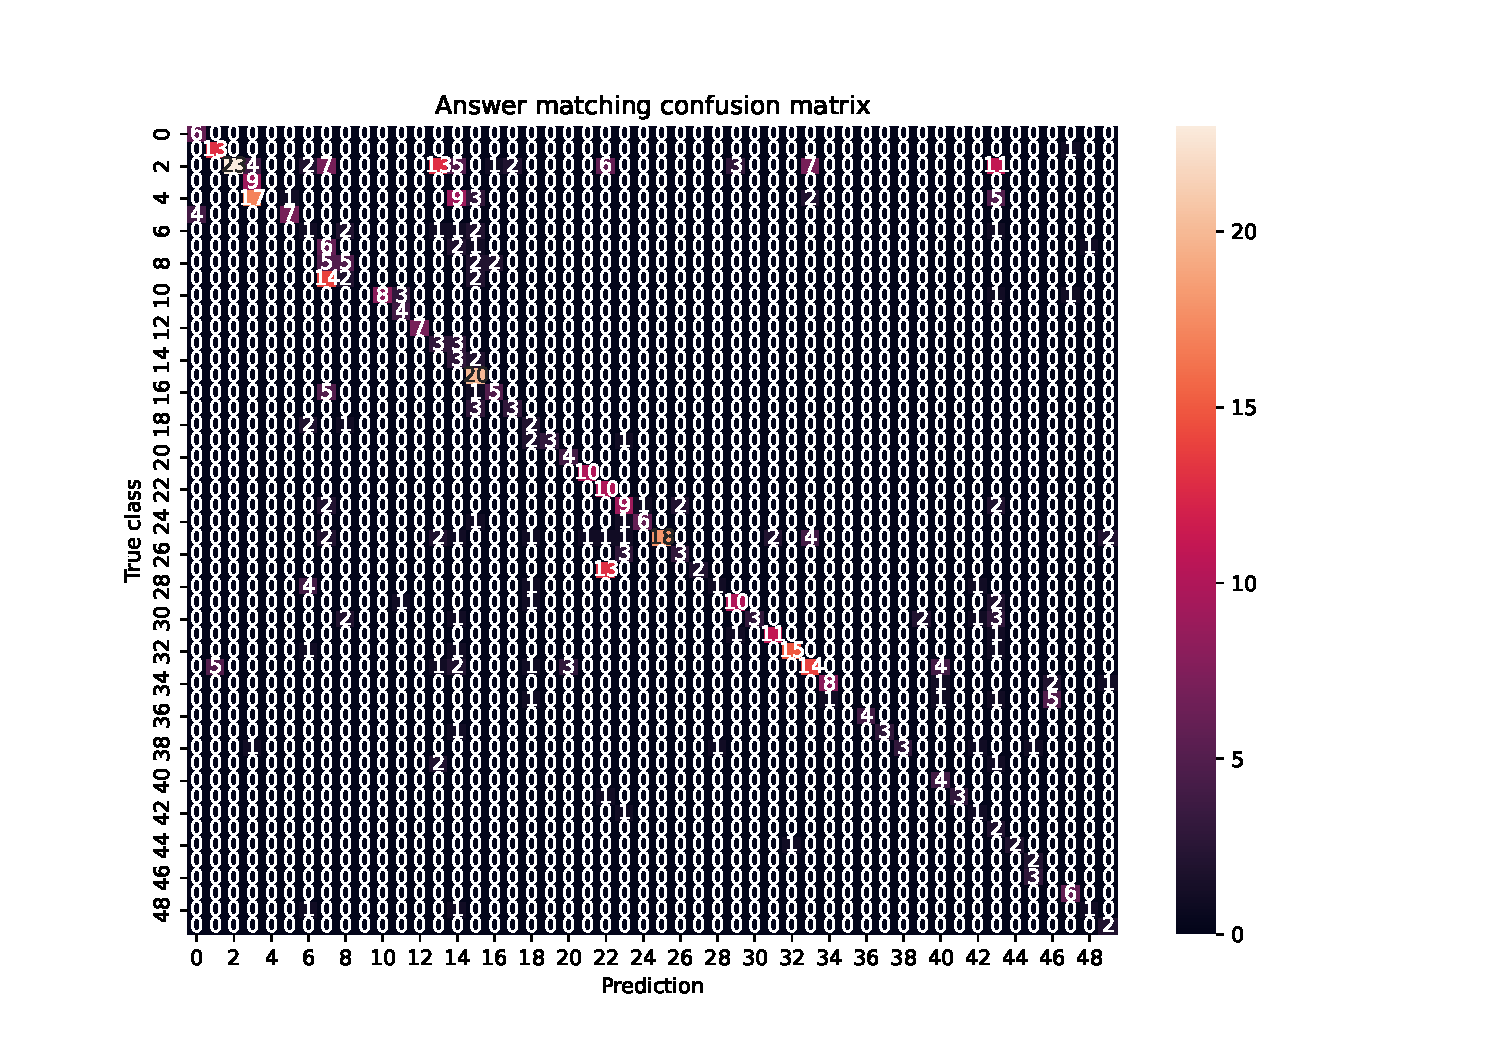
\includegraphics[width=0.54\textwidth,valign=t]{src/fig/pdfs/CM_AMA_FAQ50_diacriticless.pdf}
        \label{fig:CM_diacriticless}
    }

    \caption{Confusion matrices of \ac{mE5}\textsubscript{Large} evaluated using diacritics (a) and diacriticless (b) FAQ50 subsets of UPV FAQ dataset.}
    \label{fig:Confusion_matrices}
\end{figure}

\FloatBarrier

\begin{table*}[ht!]
  \centering
  \begin{tabular}{lcccccc}
    \toprule
    \textbf{Model} & \textbf{QMA}\textsubscript{d} & \textbf{AMA}\textsubscript{d} & \textbf{QMA}\textsubscript{dl} & \textbf{AMA}\textsubscript{dl} & \textbf{\#params} \\
    \hline
    \multicolumn{6}{c}{BASELINE} \\
    \hline
    FastText\textsubscript{diacritics} & 0.8304 & 0.2899 & 0.8110 & 0.2923 & 240M \\
    FastText\textsubscript{diacriticless} & 0.8331 & 0.2864 & 0.8320 & 0.3020 & 229M \\
    \hline
    \multicolumn{6}{c}{CZECH MODELS} \\
    \hline
    Czert-B & 0.8759 & 0.2469 & 0.8388 & 0.0977 & 110M \\
    RetroMAE-Small & 0.8651 & 0.2893 & 0.8634 & 0.2437 & 24M \\
    Dist-MPNet-ParaCrawl & 0.8540 & 0.1089 & 0.8344 & 0.0808 & 24M \\
    Dist-MPNet-CzEng & 0.8705 & 0.0487 & 0.8322 & 0.0426 & 24M \\
    SimCSE-RetroMAE-Small & 0.8682 & 0.3647 & 0.8649 & 0.3316 & 24M \\
    SimCSE-Dist-MPNet-ParaCrawl & 0.8817 & 0.2552 & 0.8602 & 0.2322 & 24M \\
    SimCSE-Dist-MPNet-CzEng & 0.8833 & 0.2278 & 0.8556 & 0.1450 & 24M \\
    SimCSE-Small-E-Czech & 0.8094 & 0.1074 & 0.8160 & 0.0878 & 13M \\
    \hline
    \multicolumn{6}{c}{MULTILINGUAL MODELS} \\
    \hline
    mBERT & 0.8584 & 0.2012 & 0.8361 & 0.1306 & 178M \\
    mE5\textsubscript{Small} & 0.8952 & 0.6078 & 0.8564 & 0.4446 & 118M \\
    mE5\textsubscript{Base} & 0.8961 & 0.6019 & 0.8726 & 0.5134 & 278M \\
    mE5\textsubscript{Large} & \textbf{0.9084} & \textbf{0.6559} & \textbf{0.8944} & \textbf{0.5593} & 560M \\
    LaBSE & 0.8875 & 0.3525 & 0.8594 & 0.3264 & 471M \\
    XLM-R\textsubscript{Base} & 0.8011 & 0.0098 & 0.7701 & 0.0198 & 279M \\
    XLM-R\textsubscript{Large} & 0.7884 & 0.0460 & 0.7411 & 0.0298 & 560M \\
    Distiluse-Base-Multilingual-Cased-v2 & 0.8335 & 0.2978 & 0.7784 & 0.2369 & 135M \\
    Paraphrase-Multilingual-MiniLM-L12-v2 & 0.8502 & 0.4062 & 0.8029 & 0.2576 & 118M \\
    Paraphrase-Multilingual-MPNet-Base-v2 & 0.8752 & 0.4538 & 0.8354 & 0.3174 & 278M \\
    \hline
    \multicolumn{6}{c}{MONOLINGUAL MODELS} \\
    \hline
    UAE-Large-V1 & 0.8241 & 0.2913 & 0.8237 & 0.2931 & 335M \\
    Mxbai-Embed-Large-v1 & 0.8308 & 0.2998 & 0.8302 & 0.2994 & 335M \\
    Mxbai-Embed-2D-Large-v1 & 0.8260 & 0.2511 & 0.8260 & 0.2516 & 335M \\
    Nomic-Embed-v1 & 0.8523 & 0.3553 & 0.8541 & 0.3751 & 137M \\
    Nomic-Embed-v1.5 & 0.8513 & 0.3537 & 0.8520 & 0.3533 & 137M \\
    Ember-v1 & 0.8259 & 0.2971 & 0.8253 & 0.2966 & 335 \\
    GTE\textsubscript{Small} & 0.8549 & 0.3632 & 0.8543 & 0.3634 & 33M \\
    GTE\textsubscript{Base} & 0.8443 & 0.3645 & 0.8437 & 0.3643 & 109M \\
    GTE\textsubscript{Large} & 0.8376 & 0.3345 & 0.8370 & 0.3352 & 335M \\
    GTE-v1.5\textsubscript{Base} & 0.8501 & 0.3336 & 0.8499 & 0.3305 & 137M \\
    GTE-v1.5\textsubscript{Large} & 0.8592 & 0.3294 & 0.8586 & 0.3289 & 434M \\
    BGE-v1.5\textsubscript{Small} & 0.8479 & 0.3816 & 0.8474 & 0.3798 & 33M \\
    BGE-v1.5\textsubscript{Base} & 0.8368 & 0.3246 & 0.8362 & 0.3240 & 109M \\
    BGE-v1.5\textsubscript{Large} & 0.8244 & 0.2938 & 0.8238 & 0.2955 & 335M \\
    GIST-Embedding-v0\textsubscript{Small} & 0.8498 & 0.2664 & 0.8493 & 0.2653 & 33M \\
    GIST-Embedding-v0\textsubscript{Base} & 0.8307 & 0.3023 & 0.8307 & 0.3023 & 109M \\
    GIST-Embedding-v0\textsubscript{Large} & 0.8219 & 0.2579 & 0.8213 & 0.2588 & 335M \\
    TaylorAI/BGE-micro-v2 & 0.8476 & 0.3616 & 0.8475 & 0.3616 & 17M \\
    TaylorAI/GTE-tiny & 0.8492 & 0.3343 & 0.8488 & 0.3342 & 23M \\
    \bottomrule
  \end{tabular}
  \caption{\textbf{Evaliation of models.}
    We show evaluation results where:
    \textbf{QMA}\textsubscript{d} (\textbf{QMA}\textsubscript{dl}) are Question Match Accuracy for the diacritics (diacriticless) model.
    \textbf{AMA}\textsubscript{d} (\textbf{AMA}\textsubscript{d}) are Question Match Accuracy for the diacritics (diacriticless) model.
    \textbf{\#params} is total number of parameters.}
  \label{tab:evaluatinon}
\end{table*}
  

\FloatBarrier

\subsection{Balanced models}
To ensure the effectiveness of the evaluation process, a selection criterion was applied to the initial set of candidate models.
This criterion focused on Question Matching Accuracy and Answer Matching Accuracy for both diacritic and diacriticless models.
Models that exhibited performance below the established baseline for their respective category (diacritic or diacriticless) were excluded from further evaluation.

Additionally, models with lower performance metrics were removed if a smaller, more efficient model demonstrated comparable or superior accuracy.
This approach ensures that the final selection of models for evaluation represents a balance between effectiveness and efficiency.

\begin{table*}[ht!]
    \centering
    \begin{tabular}{lcccccc}
      \toprule
      \textbf{Model} & \textbf{QMA}\textsubscript{d} & \textbf{AMA}\textsubscript{d} & \textbf{QMA}\textsubscript{dl} & \textbf{AMA}\textsubscript{dl} & \textbf{\#params} \\
      \midrule
      SimCSE-RetroMAE-Small & 0.8682 & 0.3647 & 0.8649 & 0.3316 & 24M \\
      GTE\textsubscript{Small} & 0.8549 & 0.3632 & 0.8543 & 0.3634 & 33M \\
      mE5\textsubscript{Small} & 0.8952 & 0.6078 & 0.8564 & 0.4446 & 118M \\
      mE5\textsubscript{Base} & 0.8961 & 0.6019 & 0.8726 & 0.5134 & 278M \\
      mE5\textsubscript{Large} & \textbf{0.9084} & \textbf{0.6559} & \textbf{0.8944} & \textbf{0.5593} & 560M \\

      
      \bottomrule
    \end{tabular}
    \caption{\textbf{Balanced models.}
    We show most factual models according to their efficiency, where:
    \textbf{QMA}\textsubscript{d} (\textbf{QMA}\textsubscript{dl}) are Question Match Accuracy for the diacritics (diacriticless) model.
    \textbf{AMA}\textsubscript{d} (\textbf{AMA}\textsubscript{d}) are Question Match Accuracy for the diacritics (diacriticless) model.
    \textbf{\#params} is total number of parameters.}
    \label{tab:balanced}
  \end{table*}
  

\section{RAG Optimization}

\begin{table*}[ht!]
    \centering
    \begin{tabular}{lc|ccc}
      \toprule
      $S_{chunk}$ & $K$ & ACC & $t_{encoding}$ \\
      \midrule
      256  & 12 & N/A & 26m 46s \\
      512  & 6  & N/A & 34m 14s \\
      1024 & 3  & N/A & N/A \\
      2048 & 2  & N/A & N/A \\
      4096 & 1  & N/A & N/A \\
      \bottomrule
    \end{tabular}
    \caption{\textbf{RAG evaluation with different parameters.}}
    \label{tab:RAG_evaluation}
  \end{table*}
  

\section{TODO: REMOVE Experiments structure}
\begin{itemize}
    \item Present the results of the evaluation for different text representations using analogy tests and confusion matrices.
    \item Discuss the findings regarding the effectiveness of each representation model for capturing semantic relationships in technical text.
    \item Analyze the results from the RAG evaluation, highlighting the impact of different representations and text chunk sizes on answer generation quality and CPU efficiency.
    \item Identify the representation model that achieves a balance between factuality of answers and computational demands.
\end{itemize}


%% --------------------------------------------------------------
%% |                         Discussion                         |
%% --------------------------------------------------------------

%!TEX root = ../main.tex

\chapter{Discussion DRAFT\label{chap:discussion}}

\section{Findings}
This study demonstrates the potential advantages of transformer-based models for text representation compared to traditional models like fastText.
Notably, the SimCSE-RetroMAE-Small transformer model achieved superior performance despite having significantly fewer parameters compared to fastText.
This suggests that the architectural design of transformer models may be particularly well-suited for capturing semantic meaning within text data.

Furthermore, the study revealed that certain monolingual models, even those not specifically trained on the Czech language used for evaluation, achieved surprisingly positive results.
This suggests that some level of semantic similarity can be captured between languages that share structural similarities, even without targeted training.
However, it is crucial to acknowledge that these models may not achieve optimal performance for tasks involving Czech text.

Finally, the study observed that unsupervised training methods employed by some models (e.g., \ac{MLM} and \ac{NSP}) resulted in lower performance compared to supervised training approaches.
This suggests that supervised training on high-quality, task-specific datasets may be necessary to achieve optimal performance in tasks involving semantic similarity assessment.


\section{Strengths and limitations of the chosen evaluation methods}

\section{Improvements for future research}
This study exclusively employed pre-trained models for the evaluation process.
While these models achieved promising results, a potential avenue for future research lies in fine-tuning the models specifically for the task of assessing semantic similarity in Czech text.



We use English dataset for \ac{RAG}  evaluation in out work.
Optimal chunk size for Czech and English languages can vary, because of different sizes of average words. 
So good idea for the future research is creation of the new dataset for technical \ac{QA} and testing for the optimal chunk size.

This study employs the K parameter within the \ac{RAG} evaluation process.
The initial K values were chosen to be proportional to the chunk size, similar to the default settings within the evaluator tool.
However, to ensure optimal performance for the \ac{QA} task, it is recommended to further investigate the impact of varying K values.
Evaluating a broader range of K values alongside the chunk size variations will enable the identification of the optimal configuration for maximizing RAG's performance within the context of this specific English technical document retrieval task.

\section{TODO: REMOVE DISCUSSION STRUCTURE}
\begin{itemize}
    \item Interpret the overall findings and their implications for choosing suitable text representations for RAG in technical QA tasks.
    \item Discuss the strengths and limitations of the chosen evaluation methods.
    \item Address potential challenges encountered during the study and suggest improvements for future research.
\end{itemize}






%% --------------------------------------------------------------
%% |                         Conclusion                         |
%% --------------------------------------------------------------

%!TEX root = ../main.tex

\chapter{Conclusion \label{chap:conclusion}}

This thesis investigated the effectiveness of transformer-based models for text representation compared to traditional methods in the context of semantic similarity assessment for Czech text.

The analysis began with a comprehensive review of traditional text representation methods.
Their architectures, underlying principles, strengths, weaknesses, and specific applications were examined.
This review established a foundation for understanding the evolution of text representation techniques.

Following this, the study shifted its focus to transformer architectures.
Here, the investigation delved into the inner workings of these models and explored their advantages over traditional methods.
The \ac{BERT} model served as a specific example, with an explanation of its training process and its strengths in capturing semantic meaning from textual data.

To ensure objective assessment of model quality for the chosen task, two relevant evaluation methods were reviewed.
These established methods provided a framework for comparing the performance of different text representation models used for semantic similarity assessment in Czech text.

Next, the investigation explored the \ac{RAG} model.
Core concepts, operational principles, and critical parameters influencing \ac{RAG}'s accuracy were examined.
This in-depth analysis proved crucial for effectively configuring and evaluating \ac{RAG} within the context of the chosen task.

Recognizing the importance of language-specific analysis, Czech was chosen as the target language.
The study incorporated both diacritic and diacritic-less text versions to account for potential variations within Czech text data.
The established UPV FAQ benchmark served as the standard for consistent and reliable evaluation.

A baseline performance metric was established using the FastText model.
This baseline provided a benchmark for comparing the performance of the transformer-based models.
Following the establishment of this baseline, a diverse selection of 15 transformer-based model groups (encompassing a total of 37 models) were chosen for further evaluation.

The \ac{RAG} evaluation process involved testing five different chunk sizes.
This exploration aimed to understand the impact of chunk size on both the factuality (accuracy) of retrieved information and computational efficiency (processing time).
The initial stage focused on selecting optimal text representation models.
We employed \ac{GTE}\textsubscript{Small} for embedding generation and GPT-3.5-turbo for answer generation.
GPT-4o was used in a separate process to assess the quality of answers generated by GPT-3.5-turbo.

After we made evaluation of the chosen models to detect best text representation models.
The evaluation results revealed that a significant portion of the transformer-based models outperformed the baseline, suggesting their promise for semantic similarity assessment in Czech text.
A detailed analysis of model performance and influencing factors identified \ac{mE5} \textsubscript{Large} as the top performer.
A confusion matrix visualized its evaluation on a specific benchmark subset.
Additionally, "balanced models" exhibiting the best performance relative to their model size were highlighted.
These included SimCSE-RetroMAE-Small, the small version of \ac{GTE}, and all sizes of \ac{mE5}, demonstrating the potential of both large and efficient models for this task.

The evaluation then proceeded to analyze the impact of chunk size on the \ac{RAG} model itself.
The first stage involved calculating the average time required for embedding generation with different chunk sizes using \ac{GTE}\textsubscript{Small}.
This analysis aimed to identify potential variations in processing time based on chunk size.
The results yielded unexpected findings, which were subsequently interpreted as a potential consequence of improved transformer model parallelism when handling larger sequences of tokens.

Following the analysis of processing time, the study investigated the impact of chunk size on model accuracy.
Based on the evaluation results, a chunk size of 4096 characters was identified as optimal for the \ac{RAG} model.


% \section{CONCLUSION STRUCTURE}
% \begin{itemize}
%     \item Summarize the key takeaways from the research, emphasizing the most effective text representation model for \ac{RAG} in technical \ac{QA} based on the evaluation criteria.
%     \item Briefly mention the trade-offs between factuality, CPU usage, and other factors in selecting representations for \ac{RAG}.
%     \item Suggest potential future research directions, such as exploring other text representation methods or evaluating \ac{RAG} performance on different datasets.
% \end{itemize}


%% --------------------------------------------------------------
%% |                         References                         |
%% --------------------------------------------------------------

\chapter{References}

\printbibliography[heading=none,title={}]

%% --------------------------------------------------------------
%% |                         Appendices                         |
%% --------------------------------------------------------------

\appendix
\renewcommand\chaptername{Appendix}

\renewcommand{\thechapter}{A}
\renewcommand\chaptername{Appendix A}

%!TEX root = ../main.tex

\chapter{Appendix A} \label{chap:appendix_A}

\reftab{tab:parameters} presents a comparison of the architectural characteristics of the evaluated text embedding models.
This table includes the following parameters for each model:

\begin{itemize}
    \item \textbf{Number of Layers ($L$)}:
 This refers to the number of encoder or decoder layers stacked within the model architecture.
 A higher number of layers typically indicates a more complex model with a greater capacity to learn complex relationships within the data.
    \item \textbf{Number of Hidden States ($H_m$)}:
 This represents the dimensionality of the internal representations processed by each layer within the model.
 A larger number of hidden states allows the model to capture a richer set of features from the input data.
    \item \textbf{Dimension of Feed-Forward Layer ($H_{ff}$)}:
 This parameter specifies the dimensionality of the hidden layer within the feed-forward sub-layer of each transformer encoder block.
 The feed-forward sub-layer allows the model to learn non-linear relationships between input features.
    \item \textbf{Number of Attention Heads ($A$)}:
 This refers to the number of parallel attention mechanisms employed within each encoder or decoder layer.
 A higher number of attention heads allows the model to focus on different aspects of the input data simultaneously.
    \item \textbf{Dimension of Output Embedding ($D$)}:
 This specifies the dimensionality of the final vector representation generated by the model for each input text sequence.
    \item \textbf{Maximum Sequence Length ($T_{max}$)}:
 This parameter indicates the maximum number of tokens a model can process within a single input sequence.
 Models with a larger $T_{max}$ can handle longer text inputs without requiring truncation.
    \item \textbf{Vocabulary Size ($V$)}:
 This represents the total number of unique words (tokens) the model's vocabulary encompasses.
    \item \textbf{Total Number of Parameters ($N_p$)}:
 This denotes the total number of trainable parameters within the model.
 A larger number of parameters typically indicates a more complex model with greater capacity, but also higher computational demands.
\end{itemize}


For Transformer encoders, the number of parameters can be approximated by Eq.~\refeq{eq:model_params}.
\begin{equation}
    \label{eq:model_params}
 N_p \approx 4LH_m^2 + 2LH_m H_{ff} + VH_m.
\end{equation}


\begin{table*}[ht!]
    \centering
    \begin{tabular}{lcccccccc}
      \toprule
      \textbf{Model} & $L$ & $H_m$ & $H_{ff}$ & $A$ & $D$ & $T_{max}$ & $V$ & $N_p$ \\
      \midrule
      Czert-B & 12 & 768 & 3072 & 12 & 768 & 512 & 31K & 110M \\
      RetroMAE-Small & 12 & 256 & 1024 & 4 & 256 & 512 & 58K & 24M \\
      Dist-MPNet-ParaCrawl & 12 & 256 & 1024 & 4 & 256 & 512 & 58K & 24M \\
      Dist-MPNet-CzEng & 12 & 256 & 1024 & 4 & 256 & 512 & 58K & 24M \\
      SimCSE-RetroMAE-Small & 12 & 256 & 1024 & 4 & 256 & 512 & 58K & 24M \\
      SimCSE-Dist-MPNet-ParaCrawl & 12 & 256 & 1024 & 4 & 256 & 512 & 58K & 24M \\
      SimCSE-Dist-MPNet-CzEng & 12 & 256 & 1024 & 4 & 256 & 512 & 58K & 24M \\
      SimCSE-Small-E-Czech & 12 & 256 & 1024 & 4 & 256 & 512 & 31K & 13M \\
      mBERT & 12 & 768 & 3072 & 12 & 768 & 512 & 120K & 178M \\
      mE5\textsubscript{Small} & 12 & 384 & 1536 & 12 & 384 & 512 & 250K & 118M \\
      mE5\textsubscript{Base} & 12 & 768 & 3072 & 12 & 768 & 514 & 250K & 278M \\
      mE5\textsubscript{Large} & 24 & 1024 & 4096 & 16 & 1024 & 514 & 250K & 560M \\
      LaBSE & 12 & 768 & 3072 & 12 & 768 & 512 & 502K & 471M \\
      XLM-R\textsubscript{Base} & 12 & 768 & 3072 & 12 & 768 & 514 & 250K & 279M \\
      XLM-R\textsubscript{Large} & 24 & 1024 & 4096 & 16 & 1024 & 514 & 250K & 560M \\
      Distiluse-Base-Multilingual-Cased-v2 & 6 & 768 & 3072 & 12 & 512 & 512 & 120K & 135M \\
      Paraphrase-Multilingual-MiniLM-L12-v2 & 12 & 384 & 1536 & 12 & 384 & 512 & 250K & 118M \\
      Paraphrase-Multilingual-MPNet-base-v2 & 12 & 768 & 3072 & 12 & 768 & 514 & 250K & 278M \\
      UAE-Large-V1 & 24 & 1024 & 4096 & 16 & 1024 & 512 & 31K & 335M \\
      Mxbai-Embed-Large-v1 & 24 & 1024 & 4096 & 16 & 1024 & 512 & 31K & 335M \\
      Mxbai-Embed-2D-Large-v1 & 24 & 1024 & 4096 & 16 & 1024 & 512 & 31K & 335M \\
      Nomic-Embed-v1 & 12 & 768 & 3072 & 12 & 768 & 8192 & 31K & 137M \\
      Nomic-Embed-v1.5 & 12 & 768 & 3072 & 12 & 768 & 8192 & 31K & 137M \\
      Ember-v1 & 24 & 1024 & 4096 & 16 & 1024 & 512 & 31K & 335M \\
      GTE\textsubscript{Small} & 12 & 384 & 1536 & 12 & 384 & 512 & 31K & 33M \\
      GTE\textsubscript{Base} & 12 & 768 & 3072 & 12 & 768 & 512 & 31K & 109M \\
      GTE\textsubscript{Large} & 24 & 1024 & 4096 & 16 & 1024 & 512 & 31K & 335M \\
      GTE-v1.5\textsubscript{Base} & 12 & 768 & 3072 & 12 & 768 & 8192 & 31K & 137M \\
      GTE-v1.5\textsubscript{Large} & 24 & 1024 & 4096 & 16 & 1024 & 8192 & 31K & 434M \\
      BGE-v1.5\textsubscript{Small} & 12 & 384 & 1536 & 12 & 384 & 512 & 31K & 33M \\
      BGE-v1.5\textsubscript{Base} & 12 & 768 & 3072 & 12 & 768 & 512 & 31K & 109M \\
      BGE-v1.5\textsubscript{Large} & 24 & 1024 & 4096 & 16 & 1024 & 512 & 31K & 335M \\
      GIST-Embedding-v0\textsubscript{Small} & 12 & 384 & 1536 & 12 & 512 & 512 & 31K & 33M \\
      GIST-Embedding-v0\textsubscript{Base}  & 12 & 768 & 3072 & 12 & 768 & 512 & 31K & 109M \\
      GIST-Embedding-v0\textsubscript{Large} & 24 & 1024 & 4096 & 16 & 1024 & 512 & 31K & 335M \\
      TaylorAI/BGE-micro-v2 & 3 & 384 & 1536 & 12 & 512 & 512 & 31K & 17M \\
      TaylorAI/GTE-tiny & 6 & 384 & 1536 & 12 & 384 & 512 & 31K & 23M \\
      \bottomrule
    \end{tabular}
    \caption{\textbf{Details on model sizes.}
            We show the number of layers $L$, the number of hidden states of the model $H_{m}$, the dimension of the feed-forward layer $H_{ff}$, the number of attention heads $A$, the dimension of output embedding $D$, the size of the vocabulary $V$ and the total number of parameters $N_p$. 
            For Transformer encoders, the number of parameters can be approximated by $4LH_m^2 + 2LH_m H_{ff} + VH_m$.
            While this table gives more hindsight on the difference of capacity of each model, note it does not highlight other critical differences between the models.}
    \label{tab:parameters}
  \end{table*}
  

\end{document}
